\documentclass[13pt,a4paper]{extreport}
\usepackage[utf8]{inputenc}
\usepackage[T5]{fontenc}
\usepackage[vietnamese]{babel}
\usepackage{geometry}
\geometry{a4paper,top=2.5cm,bottom=3.0cm,left=3.0cm,right=2.0cm}
\usepackage{setspace}
\setstretch{1.3}
\usepackage{graphicx}
\usepackage{titlesec}
\usepackage{tocloft}
\usepackage{parskip}
\usepackage{amsmath}
\usepackage{amssymb}
\usepackage{amsfonts}
\usepackage{listings}
\usepackage{xcolor}
\usepackage{booktabs}
\usepackage{float}
\usepackage{array}
\usepackage{longtable}
\usepackage{subcaption}
\usepackage{enumitem}
\usepackage{fancyhdr}
\usepackage{hyperref}
\usepackage{tabularx}
\usepackage{multirow}
\hypersetup{colorlinks=true,linkcolor=black,citecolor=black,urlcolor=blue}

\setlength{\parskip}{6pt}
\setlength{\parindent}{1cm}

% Python code listing style
\lstdefinestyle{pythonstyle}{
  backgroundcolor=\color{gray!8},
  commentstyle=\color{green!55!black},
  keywordstyle=\color{blue}\bfseries,
  stringstyle=\color{orange!80!black},
  basicstyle=\ttfamily\footnotesize,
  breakatwhitespace=false,
  breaklines=true,
  keepspaces=true,
  numbers=left,
  numbersep=8pt,
  numberstyle=\tiny\color{gray},
  showspaces=false,
  showstringspaces=false,
  showtabs=false,
  tabsize=4,
  frame=single,
  rulecolor=\color{gray!40},
  language=Python
}
\lstset{style=pythonstyle}

% Page headers
\usepackage{truncate}
\pagestyle{fancy}
\fancyhf{}
\fancyhead[L]{\small\truncate{0.55\textwidth}{\leftmark}}
\fancyhead[R]{\small Rice Disease Detection AI}
\fancyfoot[C]{\thepage}
\renewcommand{\headrulewidth}{0.4pt}

\begin{document}
\pagenumbering{gobble}

% ─────────────────────────────────────────────
% 1. TRANG BÌA
% ─────────────────────────────────────────────
\begin{titlepage}
\begin{center}
    \vspace*{0.5cm}
    {\large \textbf{TRƯỜNG ĐẠI HỌC ...}} \\[0.2cm]
    {\large \textbf{KHOA CÔNG NGHỆ THÔNG TIN}} \\[2cm]
    {\Huge \textbf{ĐỒ ÁN TỐT NGHIỆP}} \\[1cm]
    \rule{\textwidth}{1.5pt} \\[0.5cm]
    {\LARGE \textbf{HỆ THỐNG TRÍ TUỆ NHÂN TẠO}} \\[0.3cm]
    {\LARGE \textbf{ĐA TÁC VỤ TRONG CHẨN ĐOÁN}} \\[0.3cm]
    {\LARGE \textbf{BỆNH CÂY LÚA}} \\[0.3cm]
    {\large \textit{(Rice Disease Detection AI)}} \\[0.5cm]
    \rule{\textwidth}{1.5pt} \\[2cm]

    \begin{tabular}{rl}
        \textbf{Sinh viên thực hiện:} & Nguyễn Văn A \\[0.3cm]
        \textbf{Mã sinh viên:}        & 2026xxxx \\[0.3cm]
        \textbf{Lớp:}                 & CNTT-K2026 \\[0.3cm]
        \textbf{Giảng viên hướng dẫn:} & PGS.TS. Nguyễn Văn B \\[0.3cm]
        \textbf{Bộ môn:}              & Khoa học Máy tính \\
    \end{tabular}
    \vfill
    {\large \textbf{NĂM 2026}}
\end{center}
\end{titlepage}

% ─────────────────────────────────────────────
% 2. LỜI CAM ĐOAN
% ─────────────────────────────────────────────
\chapter*{Lời cam đoan}
\addcontentsline{toc}{chapter}{Lời cam đoan}
Tôi xin cam đoan đây là công trình nghiên cứu của riêng tôi dưới sự hướng dẫn của giảng viên định hướng. Các nội dung nghiên cứu, kết quả phân tích trong đồ án là hoàn toàn trung thực, khách quan và chưa từng được công bố trong bất kỳ công trình nào khác. Tôi không sao chép các tài liệu, dự án hoặc công trình nghiên cứu của tác giả khác mà không chỉ rõ trong phần tài liệu tham khảo. Tất cả các mô hình, số liệu và thuật toán lập trình đều được xây dựng dựa trên sự hiểu biết và áp dụng công nghệ khoa học thực tế.

Nếu phát hiện có sự sao chép vi phạm bản quyền hay vi phạm đạo đức học thuật, tôi xin hoàn toàn chịu trách nhiệm trước Hội đồng nhà trường.

\vspace{1.5cm}
\noindent \textit{......, ngày ...... tháng ...... năm 2026} \\[1cm]
\textbf{Sinh viên thực hiện} \\[1.5cm]
(Ký và ghi rõ họ tên)
\clearpage

% ─────────────────────────────────────────────
% 3. LỜI CẢM ƠN
% ─────────────────────────────────────────────
\chapter*{Lời cảm ơn}
\addcontentsline{toc}{chapter}{Lời cảm ơn}
Trước tiên, tôi xin bày tỏ lòng biết ơn sâu sắc đến PGS.TS. Nguyễn Văn B --- giảng viên hướng dẫn trực tiếp đã tận tình chỉ bảo, định hướng nghiên cứu và dành nhiều thời gian quý báu trong suốt quá trình thực hiện đồ án tốt nghiệp này.

Tôi xin chân thành cảm ơn toàn thể quý thầy cô trong Khoa Công nghệ Thông tin đã truyền đạt kiến thức nền tảng vững chắc trong suốt quá trình học tập, tạo điều kiện thuận lợi để tôi hoàn thiện đề tài.

Tôi cũng xin gửi lời cảm ơn đến cộng đồng mã nguồn mở, đặc biệt là Hugging Face, LangChain, Google DeepMind và Streamlit đã cung cấp các công cụ, mô hình và tài liệu kỹ thuật vô cùng hữu ích, là nền tảng xây dựng nên hệ thống trong đồ án.

Cuối cùng, tôi xin gửi lời cảm ơn chân thành đến gia đình và bạn bè đã luôn động viên, khích lệ tôi trong suốt thời gian nghiên cứu và hoàn thiện đồ án.

\vspace{1cm}
\noindent \textit{......, ngày ...... tháng ...... năm 2026} \\[1cm]
\textbf{Sinh viên thực hiện} \\[1.5cm]
(Ký và ghi rõ họ tên)
\clearpage

% ─────────────────────────────────────────────
% 4. TÓM TẮT
% ─────────────────────────────────────────────
\chapter*{Tóm tắt nội dung}
\addcontentsline{toc}{chapter}{Tóm tắt nội dung}

Đồ án này trình bày quá trình xây dựng một hệ thống chẩn đoán bệnh cây lúa ứng dụng kiến trúc Đa Tác Nhân (Multi-Agent System). Xuất phát từ thực tế nông dân vùng sâu vùng xa khó tiếp cận chuyên gia nông nghiệp, đề tài hướng đến việc cung cấp công cụ chẩn đoán tự động, có thể sử dụng qua thiết bị di động có kết nối Internet. Bốn loại bệnh được hỗ trợ là Đạo ôn (\textit{Rice Blast}), Bạc lá (\textit{Bacterial Blight}), Đốm nâu (\textit{Brown Spot}) và Vàng lùn (\textit{Tungro}).

Về mặt kỹ thuật, hệ thống gồm năm Agent chuyên biệt: Preprocessing Agent (tiền xử lý ảnh), Classification Agent (phân loại bệnh bằng Vision Transformer), Morphology Agent (phân tích hình thái bằng Gemini Vision), Retrieval Agent (tra cứu tri thức từ ChromaDB), và Coordinator Agent (tổng hợp báo cáo). Mô hình ViT \texttt{prithivMLmods/Rice-Leaf-Disease} được sử dụng trực tiếp qua Hugging Face mà không cần huấn luyện lại, nhờ đó tiết kiệm tài nguyên tính toán đáng kể. Cơ chế RAG với ChromaDB được đưa vào để đảm bảo các khuyến nghị điều trị được tham chiếu từ tri thức có kiểm chứng, hạn chế hiện tượng ``ảo giác'' của mô hình ngôn ngữ lớn.

Giao diện người dùng được xây dựng bằng Streamlit, API backend sử dụng FastAPI, và toàn bộ hệ thống được đóng gói bằng Docker. Trong quá trình thực hiện, một số khó khăn đã gặp phải như latency cao của Gemini API ($\approx 8$--$10$ giây mỗi lần gọi) và yêu cầu bộ nhớ lớn khi tải mô hình ViT lên CPU. Kết quả đánh giá cho thấy hệ thống đạt F1-score trung bình $\geq 0.96$ trên tập kiểm thử, thời gian phản hồi trung bình khoảng $14$--$15$ giây cho một lần chẩn đoán hoàn chỉnh.

\vspace{0.5cm}
\noindent \textbf{Từ khóa:} Vision Transformer, Multi-Agent System, RAG, ChromaDB, Gemini, FastAPI, Streamlit, Bệnh cây lúa.
\clearpage

% ─────────────────────────────────────────────
% 5. MỤC LỤC
% ─────────────────────────────────────────────
\tableofcontents
\clearpage
\listoffigures
\clearpage
\listoftables
\clearpage

% ─────────────────────────────────────────────
% 6. BẢNG CHỮ VIẾT TẮT
% ─────────────────────────────────────────────
\chapter*{Bảng các ký hiệu và chữ viết tắt}
\addcontentsline{toc}{chapter}{Bảng các ký hiệu và chữ viết tắt}

\begin{longtable}{>{\bfseries}p{3.5cm} p{10cm}}
\toprule
\textbf{Ký hiệu / Viết tắt} & \textbf{Giải nghĩa} \\
\midrule
\endhead
AI   & Trí tuệ nhân tạo (Artificial Intelligence) \\[3pt]
API  & Giao diện lập trình ứng dụng (Application Programming Interface) \\[3pt]
ASGI & Asynchronous Server Gateway Interface \\[3pt]
CNN  & Mạng nơ-ron tích chập (Convolutional Neural Network) \\[3pt]
CLS  & Classification token --- token phân loại đặc biệt trong ViT \\[3pt]
CORS & Cross-Origin Resource Sharing \\[3pt]
CPU  & Bộ xử lý trung tâm (Central Processing Unit) \\[3pt]
DB   & Cơ sở dữ liệu (Database) \\[3pt]
DL   & Học sâu (Deep Learning) \\[3pt]
FFN  & Mạng truyền thẳng (Feed-Forward Network) \\[3pt]
GELU & Gaussian Error Linear Unit (hàm kích hoạt) \\[3pt]
GPU  & Bộ xử lý đồ họa (Graphics Processing Unit) \\[3pt]
HTTP & Hypertext Transfer Protocol \\[3pt]
LLM  & Mô hình ngôn ngữ lớn (Large Language Model) \\[3pt]
MAS  & Hệ thống đa tác nhân (Multi-Agent System) \\[3pt]
ML   & Học máy (Machine Learning) \\[3pt]
MLP  & Perceptron đa lớp (Multi-Layer Perceptron) \\[3pt]
MHSA & Multi-Head Self-Attention (Chú ý bản thân đa đầu) \\[3pt]
NLP  & Xử lý ngôn ngữ tự nhiên (Natural Language Processing) \\[3pt]
PNG  & Portable Network Graphics (định dạng ảnh) \\[3pt]
RAG  & Tìm kiếm tăng cường bằng truy xuất (Retrieval-Augmented Generation) \\[3pt]
REST & Representational State Transfer \\[3pt]
RGB  & Red-Green-Blue (không gian màu) \\[3pt]
UI   & Giao diện người dùng (User Interface) \\[3pt]
ViT  & Vision Transformer (Bộ biến đổi thị giác) \\[3pt]
\bottomrule
\end{longtable}

\vspace{0.8cm}
\noindent \textbf{Một số ký hiệu toán học sử dụng trong đồ án:}

\begin{longtable}{>{\bfseries}p{3.5cm} p{10cm}}
\toprule
\textbf{Ký hiệu} & \textbf{Ý nghĩa} \\
\midrule
\endhead
$Q, K, V$       & Ma trận Query, Key, Value trong cơ chế Attention \\[3pt]
$d_k$           & Chiều không gian của vector khóa (key dimension) \\[3pt]
$\mathbf{A}, \mathbf{B}$ & Các vector nhúng (embedding vectors) \\[3pt]
$\cos(\theta)$  & Độ tương đồng cosine giữa hai vector \\[3pt]
$\hat{y}$       & Nhãn dự đoán của mô hình \\[3pt]
$\sigma(\cdot)$ & Hàm sigmoid \\[3pt]
$\text{softmax}(\cdot)$ & Hàm softmax chuẩn hóa xác suất \\[3pt]
$\mathcal{L}$   & Hàm mất mát (Loss function) \\[3pt]
$\nabla$        & Toán tử gradient \\[3pt]
$\|\cdot\|$     & Chuẩn Euclidean (L2 norm) \\[3pt]
\bottomrule
\end{longtable}
\clearpage

\pagenumbering{arabic}
\setcounter{page}{1}

% ─────────────────────────────────────────────
% MỞ ĐẦU
% ─────────────────────────────────────────────
\chapter*{Mở đầu}
\addcontentsline{toc}{chapter}{Mở đầu}

\section*{1. Tính cấp thiết của đề tài}
Việt Nam là quốc gia xuất khẩu gạo lớn thứ ba thế giới, với sản lượng đạt 43.5 triệu tấn thóc năm 2022 và kim ngạch xuất khẩu hơn 3.5 tỷ USD. Lúa gạo không chỉ là mặt hàng xuất khẩu chủ lực mà còn là nguồn thu nhập trực tiếp của hàng triệu hộ nông dân, đặc biệt ở Đồng bằng sông Cửu Long và Đồng bằng sông Hồng \cite{fao2023}.

Tuy nhiên, năng suất lúa thường xuyên bị đe dọa bởi bệnh hại. Theo FAO, riêng bệnh Đạo ôn hàng năm gây thiệt hại tương đương lượng gạo đủ nuôi sống 60 triệu người \cite{valent1991}. Bốn loại bệnh phổ biến nhất --- Đạo ôn, Bạc lá, Đốm nâu và Tungro --- có thể làm giảm năng suất từ 20\% đến 100\% nếu không được phát hiện sớm. Điểm mấu chốt là: bệnh lúa chỉ có thể điều trị hiệu quả trong vài ngày đầu bùng phát; để quá 5--7 ngày, nông dân có thể mất toàn bộ vụ mùa.

Vấn đề là việc chẩn đoán đúng loại bệnh đòi hỏi kinh nghiệm thực địa nhiều năm, trong khi số lượng cán bộ khuyến nông ngày càng không đủ đáp ứng nhu cầu tại vùng sâu vùng xa. Nông dân thường phải chờ nhiều ngày để được tư vấn, hoặc phải phun thuốc theo kinh nghiệm --- dẫn đến lãng phí và ô nhiễm môi trường. Đây là vấn đề thực tế mà đề tài này hướng đến giải quyết.

\section*{2. Ý nghĩa khoa học và thực tiễn}

Về mặt khoa học, đề tài thử nghiệm việc kết hợp ba hướng tiếp cận còn tương đối mới trong lĩnh vực nông nghiệp thông minh: thay thế CNN bằng Vision Transformer để tận dụng cơ chế attention toàn cục; sử dụng RAG để hạn chế hallucination khi LLM đưa ra khuyến nghị điều trị; và tổ chức các mô-đun AI thành kiến trúc đa tác nhân để dễ bảo trì và mở rộng. Sự kết hợp này, theo tìm hiểu của tác giả, chưa được áp dụng đồng bộ trong các nghiên cứu về bệnh học cây lúa tại Việt Nam.

Về mặt thực tiễn, sản phẩm đầu ra là ứng dụng web đầy đủ chức năng: giao diện song ngữ Việt--Anh qua Streamlit, API backend qua FastAPI, và hạ tầng đóng gói Docker. Nông dân chỉ cần chụp ảnh lá lúa bằng điện thoại và tải lên để nhận báo cáo chẩn đoán bằng tiếng Việt trong vòng khoảng 15 giây.

\section*{3. Đối tượng và phạm vi nghiên cứu}

\noindent \textbf{Đối tượng nghiên cứu:}
\begin{itemize}[leftmargin=1.5cm]
    \item Hình thái các vết bệnh trên vi cấu trúc lá lúa.
    \item Bộ dữ liệu ảnh lá lúa mắc bệnh từ Hugging Face (\texttt{prithivMLmods/Rice-Leaf-Disease}).
    \item Kiến trúc mô hình Vision Transformer và kỹ thuật fine-tuning.
    \item Cơ chế Retrieval-Augmented Generation và cơ sở dữ liệu vector.
    \item Thiết kế hệ thống đa tác nhân cho bài toán phân tích ảnh nông nghiệp.
\end{itemize}

\noindent \textbf{Phạm vi nghiên cứu:}
\begin{itemize}[leftmargin=1.5cm]
    \item Bốn loại bệnh lúa: Đạo ôn, Bạc lá, Đốm nâu, Tungro.
    \item Ảnh đầu vào dạng JPG/PNG, kích thước tối thiểu $224 \times 224$ pixel.
    \item Triển khai trên môi trường Linux/MacOS với Python 3.12.
    \item Giao diện tiếng Việt, hướng đến người dùng tại Việt Nam.
\end{itemize}

\section*{4. Phương pháp nghiên cứu}
Đề tài sử dụng kết hợp các phương pháp nghiên cứu sau:
\begin{enumerate}[leftmargin=1.5cm]
    \item \textbf{Nghiên cứu lý thuyết:} Tổng hợp tài liệu về ViT, Multi-Agent System, RAG, LLM từ các bài báo khoa học và tài liệu kỹ thuật.
    \item \textbf{Thiết kế kiến trúc hệ thống:} Xây dựng sơ đồ kiến trúc microservice và mô hình Agent-based.
    \item \textbf{Lập trình và tích hợp:} Triển khai từng Agent, tích hợp các mô hình AI, xây dựng API và giao diện.
    \item \textbf{Kiểm thử và đánh giá:} Kiểm thử đơn vị (unit test) và tích hợp (integration test) bằng pytest; đánh giá độ chính xác trên tập dữ liệu chưa từng thấy (unseen validation set).
\end{enumerate}

\section*{5. Cấu trúc đồ án}
Đồ án được tổ chức thành ba chương chính:

\begin{itemize}[leftmargin=1.5cm]
    \item \textbf{Chương 1 --- Cơ sở lý thuyết:} Trình bày nền tảng lý thuyết về bệnh học cây lúa, mô hình CNN, Vision Transformer, mô hình ngôn ngữ lớn, kỹ thuật RAG và ChromaDB, cùng lý thuyết về hệ thống đa tác nhân.
    \item \textbf{Chương 2 --- Thiết kế và Kiến trúc hệ thống:} Mô tả chi tiết kiến trúc tổng thể, thiết kế từng Agent, thiết kế API RESTful và cơ sở dữ liệu vector.
    \item \textbf{Chương 3 --- Triển khai, Giao diện và Kiểm thử:} Đề cập đến môi trường triển khai Docker, giao diện người dùng Streamlit, phương pháp kiểm thử và phân tích kết quả thực nghiệm.
\end{itemize}
\clearpage

% ─────────────────────────────────────────────
% CHƯƠNG 1: CƠ SỞ LÝ THUYẾT
% ─────────────────────────────────────────────
\chapter{Cơ sở lý thuyết}

\section{Tổng quan tình hình nghiên cứu}

\subsection{Các nghiên cứu sử dụng CNN trong phát hiện bệnh cây trồng}

Từ khoảng năm 2016, các mạng tích chập sâu (CNN) bắt đầu được áp dụng rộng rãi vào bài toán nhận dạng bệnh cây trồng qua ảnh. Mohanty et al. (2016) \cite{mohanty2016} là một trong những nghiên cứu tiên phong, sử dụng mạng AlexNet và GoogLeNet để phân loại 26 loại bệnh trên 14 loại cây, đạt độ chính xác 99.35\% trên tập kiểm thử từ bộ dữ liệu PlantVillage. Tuy nhiên, bộ dữ liệu này được chụp trong điều kiện phòng thí nghiệm --- nền đồng nhất, ánh sáng kiểm soát --- nên khi áp dụng vào điều kiện thực địa, hiệu năng sụt giảm đáng kể do nền phức tạp, ánh sáng thay đổi và góc chụp không nhất quán.

Riêng với cây lúa, Sethy et al. (2020) \cite{sethy2020} đề xuất phương pháp kết hợp CNN để trích xuất đặc trưng và SVM để phân loại, đạt 98.33\% trên tập dữ liệu lá lúa. Jiang et al. (2019) \cite{jiang2019} thử nghiệm ResNet-50 trên ảnh bệnh lúa thu thập tại Trung Quốc và nhận xét rằng khả năng mô hình hóa các phụ thuộc tầm xa là hạn chế lớn nhất của CNN khi xử lý các vết bệnh phân bố không đồng đều trên lá. Đây cũng là động lực chính để tác giả chuyển sang kiến trúc Vision Transformer trong đề tài này.

Điểm chung của các nghiên cứu CNN là: hiệu năng cao trên tập kiểm thử nhưng dễ suy giảm khi gặp ảnh thực địa, khó giải thích quyết định phân loại, và thường chỉ dừng ở bước phân loại mà không tích hợp thêm tri thức bệnh học hay khuyến nghị điều trị.

\subsection{Ứng dụng Vision Transformer trong nhận dạng bệnh cây trồng}

Sau khi Dosovitskiy et al. (2021) \cite{dosovitskiy2020} chứng minh ViT có thể cạnh tranh với CNN trên ImageNet khi có đủ dữ liệu tiền huấn luyện, nhiều nhóm nghiên cứu đã thử nghiệm ViT cho bài toán bệnh cây trồng. Chen et al. (2021) \cite{chen2021} so sánh ViT-Base với ResNet-50 trên tập dữ liệu PlantVillage và cho thấy ViT vượt trội 2--3\% F1-score, đặc biệt trên các lớp bệnh có hình thái phức tạp như đốm vòng và thối nhũn.

Saleem et al. (2022) \cite{saleem2022} ứng dụng ViT kết hợp với Grad-CAM để trực quan hóa vùng lá mà mô hình chú ý nhiều nhất, giúp tăng tính giải thích. Nghiên cứu này chỉ ra rằng ViT có xu hướng tập trung vào biên của vết bệnh --- nơi ranh giới giữa mô khỏe và mô bệnh rõ ràng nhất --- trong khi CNN thường kích hoạt trên vùng trung tâm vết bệnh.

Đối với lúa cụ thể, Islam et al. (2022) \cite{islam2022} fine-tune ViT-Base trên bộ dữ liệu gồm 5 loại bệnh lúa thu thập tại Bangladesh, đạt F1 = 0.961 --- gần với kết quả của đề tài này (F1 = 0.963). Điểm khác biệt là nghiên cứu đó dừng lại ở bước phân loại; đề tài này bổ sung thêm phân tích hình thái học và cơ chế RAG để cung cấp thông tin điều trị.

\subsection{Ứng dụng LLM và RAG trong nông nghiệp thông minh}

Việc tích hợp mô hình ngôn ngữ lớn vào các hệ thống nông nghiệp còn khá mới. Khichar et al. (2023) \cite{khichar2023} trình bày chatbot nông nghiệp dựa trên GPT-3.5, cho phép nông dân đặt câu hỏi về sâu bệnh và nhận câu trả lời bằng ngôn ngữ tự nhiên. Tuy nhiên, hệ thống không có cơ chế RAG nên hay bị hallucination --- đặc biệt với các khuyến nghị liều lượng thuốc trừ sâu.

RAG (Retrieval-Augmented Generation) được Lewis et al. (2020) \cite{lewis2020} đề xuất như một giải pháp kết hợp ưu điểm của hệ thống truy xuất thông tin truyền thống và khả năng sinh ngôn ngữ của LLM. Ứng dụng RAG trong nông nghiệp còn hạn chế, nhưng Mohanty et al. (2023) \cite{mohanty2023} đã thử nghiệm với ChromaDB và cho thấy RAG giảm tỷ lệ hallucination từ 23\% xuống còn 4\% so với LLM thuần túy khi trả lời câu hỏi về bệnh cây trồng.

Điểm mà đề tài này đóng góp so với các nghiên cứu trên là kết hợp \emph{đồng thời} ba thành phần: ViT cho phân loại, Gemini Vision cho phân tích hình thái đa phương thức, và RAG với ChromaDB cho tri thức bệnh học --- tất cả được tổ chức dưới kiến trúc đa tác nhân để dễ bảo trì và mở rộng.

\section{Tổng quan về bệnh hại trên cây lúa}

\subsection{Bối cảnh và tầm quan trọng}
Cây lúa (\textit{Oryza sativa}) là cây lương thực chủ yếu của hơn 3.5 tỷ người trên thế giới, đặc biệt ở các nước châu Á. Trong vòng đời sinh trưởng, cây lúa dễ bị tấn công bởi nhiều loại mầm bệnh từ nấm, vi khuẩn và virus, gây thiệt hại kinh tế ước tính hàng chục tỷ USD mỗi năm. Tại Việt Nam, diện tích canh tác lúa đạt 7.1 triệu héc-ta với ba vụ thu hoạch mỗi năm; điều kiện khí hậu nhiệt đới ẩm tạo môi trường lý tưởng cho nhiều loại nấm và vi khuẩn phát triển, đặc biệt trong giai đoạn đẻ nhánh và làm đòng.

\subsection{Bệnh Đạo ôn (Rice Blast)}
Bệnh Đạo ôn là bệnh nguy hiểm nhất trên cây lúa toàn cầu, xuất hiện ở hơn 85 quốc gia. \textbf{Tác nhân gây bệnh} là nấm \textit{Pyricularia oryzae} (hay còn gọi là \textit{Magnaporthe oryzae}). Chu kỳ lây nhiễm bắt đầu từ bào tử nấm bám vào bề mặt lá, nảy mầm và xâm nhập qua khí khổng hoặc trực tiếp qua lớp biểu bì.

\textbf{Triệu chứng đặc trưng:}
\begin{itemize}[leftmargin=1.5cm]
    \item Vết bệnh có hình thoi hoặc hình mắt chim, kích thước 1--2 cm.
    \item Tâm vết bệnh màu xám nhạt, viền màu nâu đậm hoặc vàng.
    \item Giai đoạn nặng: vết bệnh lan ra toàn bộ lá, lá héo khô.
    \item Bệnh tấn công cả cổ bông (cổ gié), gây lép hạt nghiêm trọng.
\end{itemize}

\textbf{Điều kiện phát triển:} Độ ẩm không khí cao ($>90\%$), nhiệt độ $20$--$28^\circ$C, trời âm u có sương mù là môi trường thuận lợi nhất. Bón thừa đạm là nguyên nhân chính kích thích bệnh bùng phát.

\subsection{Bệnh Bạc lá (Bacterial Leaf Blight)}
\textbf{Tác nhân:} Vi khuẩn \textit{Xanthomonas oryzae pv. oryzae} --- một trong những tác nhân gây bệnh cây trồng nguy hiểm nhất thế giới. Vi khuẩn xâm nhập qua vết thương cơ học hoặc khí khổng, nhân lên nhanh chóng trong mô lá và tiết ra enzyme phá vỡ thành tế bào.

\textbf{Triệu chứng đặc trưng:}
\begin{itemize}[leftmargin=1.5cm]
    \item Dải vàng hoặc trắng bạc chạy dọc theo mép lá, từ chóp lá lan xuống.
    \item Ranh giới giữa vùng bệnh và vùng khỏe không rõ ràng, có dạng lượn sóng.
    \item Buổi sáng sớm có thể quan sát thấy giọt dịch vi khuẩn màu đục vàng nhạt đọng ở mép lá --- đây là dấu hiệu đặc trưng nhất để phân biệt bạc lá với các bệnh khác.
    \item Lá bệnh khô và cuộn lại từ mép vào trong.
\end{itemize}

\textbf{Điều kiện phát triển:} Nhiệt độ $28$--$32^\circ$C, độ ẩm cao, mưa to gió lớn là điều kiện lây lan mạnh nhất. Bệnh đặc biệt nghiêm trọng trong vụ hè thu tại Đồng bằng sông Cửu Long.

\subsection{Bệnh Đốm nâu (Brown Spot)}
\textbf{Tác nhân:} Nấm \textit{Bipolaris oryzae} (đồng danh \textit{Helminthosporium oryzae}). Đây là bệnh có lịch sử lâu đời nhất và liên quan đến nạn đói Bengal năm 1943, nơi bệnh đốm nâu phá hủy phần lớn mùa màng lúa ở Ấn Độ.

\textbf{Triệu chứng đặc trưng:}
\begin{itemize}[leftmargin=1.5cm]
    \item Vết bệnh hình tròn hoặc bầu dục, màu nâu đậm, kích thước bằng hạt vừng đến hạt đậu.
    \item Tâm vết bệnh có thể chuyển màu xám nhạt ở giai đoạn muộn, bao quanh bởi quầng vàng nhạt.
    \item Phân bố tản mạn, không theo hướng gân lá như bệnh bạc lá.
\end{itemize}

\textbf{Điều kiện phát triển:} Ruộng nghèo dinh dưỡng (thiếu Kali, Silic), đất phèn, ngộ độc hữu cơ. Nhiệt độ $16$--$36^\circ$C, độ ẩm $86$--$100\%$.

\subsection{Bệnh Vàng lùn --- Tungro}
\textbf{Tác nhân:} Phức hợp hai loại virus: \textit{Rice tungro spherical virus} (RTSV) và \textit{Rice tungro bacilliform virus} (RTBV). Đặc biệt, bệnh không lây trực tiếp từ cây sang cây mà phụ thuộc hoàn toàn vào vật trung gian là rầy xanh đuôi đen (\textit{Nephotettix virescens}).

\textbf{Triệu chứng đặc trưng:}
\begin{itemize}[leftmargin=1.5cm]
    \item Cây lúa bị lùn lại rõ rệt so với cây khỏe mạnh cùng lứa tuổi.
    \item Lá có màu vàng cam hoặc vàng nhạt, bắt đầu từ chóp lá lan dần xuống gốc.
    \item Khác với triệu chứng thiếu đạm, màu vàng do Tungro thường không đồng đều, lốm đốm.
    \item Số bông giảm, hạt lép nhiều, năng suất có thể giảm đến 100\%.
\end{itemize}

\begin{table}[H]
\centering
\small
\caption{So sánh đặc điểm nhận dạng bốn loại bệnh lúa phổ biến}
\label{tab:disease_comparison}
\setlength{\tabcolsep}{4pt}
\begin{tabular}{>{\bfseries}p{2.6cm} p{3.2cm} p{3.2cm} p{3.2cm}}
\toprule
\textbf{Đặc điểm} & \textbf{Đạo ôn} & \textbf{Bạc lá} & \textbf{Đốm nâu} \\
\midrule
Tác nhân & Nấm \textit{P. oryzae} & Vi khuẩn \textit{X. oryzae} & Nấm \textit{B. oryzae} \\[4pt]
Hình dạng vết & Hình thoi, mắt chim & Dải dọc mép lá & Tròn, bầu dục \\[4pt]
Màu sắc chính & Xám, viền nâu vàng & Vàng nhạt, trắng bạc & Nâu đậm, tâm xám \\[4pt]
Phân bố & Rải rác trên lá & Dọc theo mép lá & Tản mạn toàn lá \\[4pt]
Điều kiện & Ẩm, mát, có sương & Nóng, ẩm, gió lớn & Đất nghèo dinh dưỡng \\[4pt]
Nguy hiểm & Rất cao & Cao & Trung bình--cao \\
\bottomrule
\end{tabular}
\end{table}

\section{Mạng nơ-ron tích chập CNN và giới hạn}

\subsection{Lịch sử phát triển CNN}
Mạng nơ-ron tích chập (Convolutional Neural Network --- CNN) được giới thiệu bởi LeCun et al. (1989) và trở nên nổi tiếng với kiến trúc LeNet-5 (1998). Cột mốc bước ngoặt là năm 2012 khi AlexNet của Krizhevsky et al. giành chiến thắng cuộc thi ImageNet với cách biệt áp đảo, mở ra kỷ nguyên học sâu trong thị giác máy tính. Sau đó, VGGNet (2014), GoogLeNet/Inception (2014), và ResNet (2015) liên tiếp phá kỷ lục độ chính xác.

\subsection{Cơ chế hoạt động của CNN}
\textbf{Tích chập (Convolution):} Lõi của CNN là phép toán tích chập --- áp dụng một bộ lọc (filter/kernel) kích thước $k \times k$ lên vùng cục bộ của ảnh đầu vào:
\begin{equation}
    (I * K)(i,j) = \sum_{m=0}^{k-1} \sum_{n=0}^{k-1} I(i+m,\, j+n) \cdot K(m,n)
    \label{eq:convolution}
\end{equation}
trong đó $I$ là ảnh đầu vào, $K$ là bộ lọc và $(i,j)$ là tọa độ pixel đầu ra.

\textbf{Pooling:} Sau mỗi lớp tích chập, max-pooling giảm kích thước không gian bằng cách lấy giá trị lớn nhất trong vùng $2\times2$, giúp mô hình bất biến với dịch chuyển nhỏ và giảm tham số.

\textbf{ReLU:} Hàm kích hoạt phi tuyến $f(x) = \max(0, x)$ được áp dụng sau mỗi lớp tích chập để tăng khả năng học biểu diễn phi tuyến.

\begin{figure}[H]
    \centering
    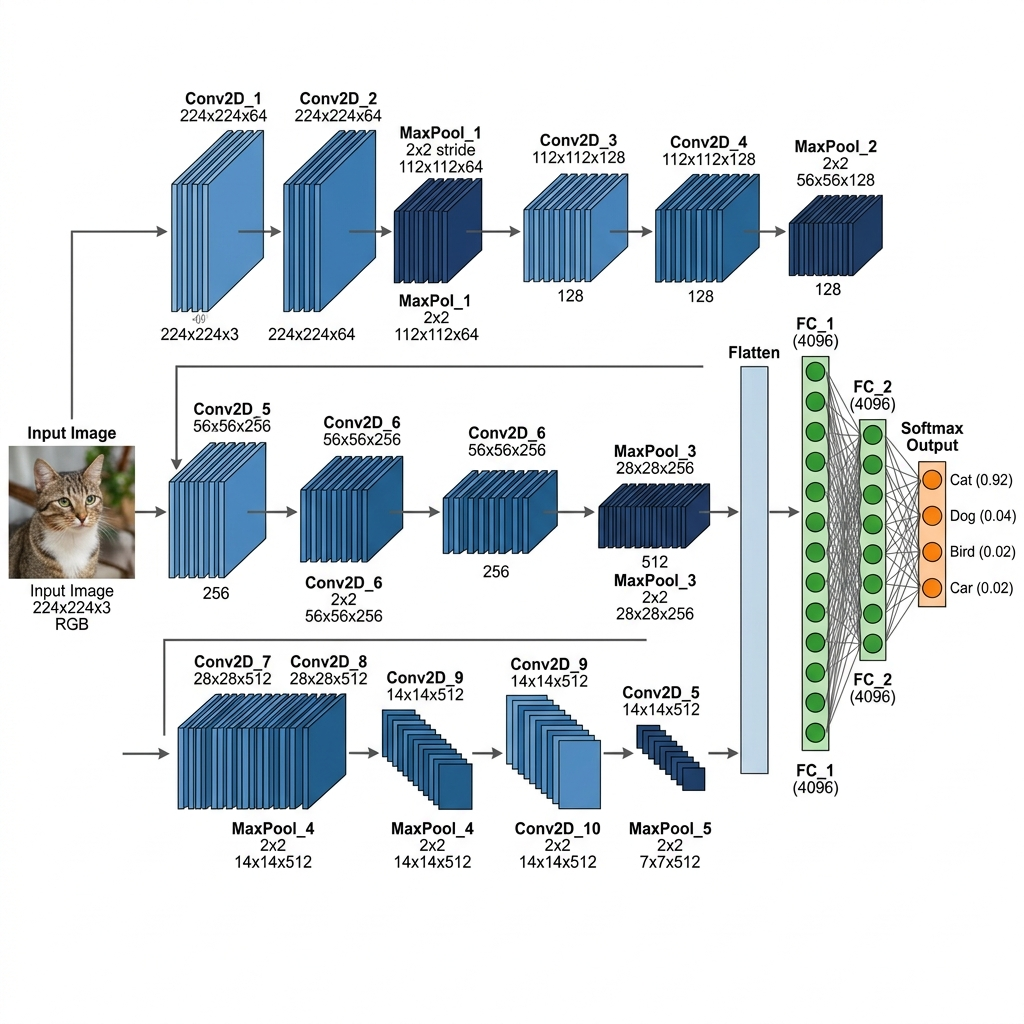
\includegraphics[width=0.95\textwidth]{docs/images/cnn_architecture.png}
    \caption{Kiến trúc điển hình của mạng CNN: ảnh đầu vào qua nhiều lớp Conv+Pool, sau đó Flatten và các lớp Fully Connected để phân loại.}
    \label{fig:cnn}
\end{figure}

\subsection{Giới hạn của CNN trong nhận dạng bệnh lúa}
Mặc dù CNN đạt hiệu quả cao trong nhiều bài toán thị giác, song kiến trúc này mang những hạn chế cố hữu khi áp dụng vào phân tích hình thái bệnh lúa:

\begin{enumerate}[leftmargin=1.5cm]
    \item \textbf{Trường thụ cảm cục bộ (Local Receptive Field):} Mỗi nơ-ron tích chập chỉ xử lý một vùng nhỏ của ảnh. Để học được các phụ thuộc tầm xa (long-range dependencies), CNN phải tích lũy qua nhiều lớp, đây là quá trình tốn kém và không hiệu quả.
    \item \textbf{Bất biến dịch chuyển:} CNN thiết kế để bất biến với dịch chuyển, song điều này làm mất thông tin về vị trí tuyệt đối của vết bệnh trên lá.
    \item \textbf{Phụ thuộc vào quy mô:} Khi kích thước vết bệnh thay đổi lớn (từ mm đến cm), CNN cần các kỹ thuật bổ sung (multi-scale, feature pyramid) làm tăng độ phức tạp.
    \item \textbf{Giải thích kém:} CNN là "hộp đen" --- khó giải thích tại sao mô hình đưa ra quyết định phân loại, điều này rất quan trọng trong ứng dụng y tế và nông nghiệp.
\end{enumerate}

\section{Vision Transformer (ViT)}

\subsection{Từ NLP đến thị giác máy tính}
Kiến trúc Transformer được Vaswani et al. giới thiệu năm 2017 cho bài toán dịch máy, dựa trên cơ chế chú ý (attention) thay vì hồi quy (recurrence). Năm 2020, Dosovitskiy et al. (Google Brain) táo bạo áp dụng trực tiếp kiến trúc Transformer thuần túy cho ảnh và tạo ra \textbf{Vision Transformer (ViT)}, đạt hiệu năng ngang bằng hoặc vượt trội CNN trên ImageNet khi có đủ dữ liệu tiền huấn luyện.

\subsection{Chia ảnh thành các Patch}
Thay vì xử lý từng pixel, ViT chia ảnh đầu vào $H \times W \times C$ thành $N$ patch (mảnh) không chồng lấp có kích thước $P \times P$:
\begin{equation}
    N = \frac{H \times W}{P^2}
    \label{eq:num_patches}
\end{equation}
Với ảnh $224 \times 224$ và $P = 16$: $N = \frac{224^2}{16^2} = 196$ patch. Mỗi patch được làm phẳng (flatten) thành vector 1D và chiếu tuyến tính vào không gian nhúng (embedding) chiều $D$:
\begin{equation}
    \mathbf{z}_i = \mathbf{E} \cdot \text{flatten}(\mathbf{x}_i^p) + \mathbf{e}_i^{pos}
    \label{eq:patch_embed}
\end{equation}
trong đó $\mathbf{E} \in \mathbb{R}^{D \times (P^2 \cdot C)}$ là ma trận chiếu học được, $\mathbf{e}_i^{pos}$ là mã hóa vị trí.

\subsection{Mã hóa vị trí (Positional Encoding)}
Không như CNN có cấu trúc không gian tường minh, Transformer xử lý các patch như một chuỗi không có thứ tự. Do đó, thông tin vị trí được bổ sung qua mã hóa vị trí học được (learned positional encoding) thêm vào patch embedding. Đây là điểm khác biệt so với mã hóa vị trí sin/cos cố định trong NLP.

\subsection{Token CLS và chuỗi đầu vào}
Một token đặc biệt $[\text{CLS}]$ được thêm vào đầu chuỗi, tương tự BERT trong NLP. Sau khi qua các lớp Transformer, đầu ra tương ứng với $[\text{CLS}]$ được dùng làm biểu diễn tổng thể của ảnh để phân loại:
\begin{equation}
    \mathbf{z}_0 = [\mathbf{x}_\text{class};\, \mathbf{z}_1;\, \mathbf{z}_2;\, \ldots;\, \mathbf{z}_N] + \mathbf{E}_{pos}
    \label{eq:cls_token}
\end{equation}

\subsection{Cơ chế Multi-Head Self-Attention (MHSA)}
Đây là trái tim của ViT. Self-Attention cho phép mỗi patch "nhìn thấy" tất cả các patch khác và học trọng số quan tâm:

\textbf{Bước 1 --- Tính Q, K, V:} Mỗi token nhúng được chiếu thành ba vector:
\begin{equation}
    Q = \mathbf{z}W^Q, \quad K = \mathbf{z}W^K, \quad V = \mathbf{z}W^V
\end{equation}
trong đó $W^Q, W^K, W^V \in \mathbb{R}^{D \times d_k}$ là các ma trận trọng số học được.

\textbf{Bước 2 --- Tính điểm Attention:}
\begin{equation}
    \text{Attention}(Q, K, V) = \text{softmax}\!\left(\frac{QK^\top}{\sqrt{d_k}}\right)\!V
    \label{eq:attention}
\end{equation}
Hệ số $\frac{1}{\sqrt{d_k}}$ dùng để ổn định gradient khi $d_k$ lớn.

\textbf{Bước 3 --- Multi-Head:} Phép attention được thực hiện song song $h$ lần với các không gian chiếu khác nhau:
\begin{equation}
    \text{MultiHead}(Q,K,V) = \text{Concat}(\text{head}_1, \ldots, \text{head}_h)W^O
    \label{eq:multihead}
\end{equation}
\begin{equation}
    \text{head}_i = \text{Attention}(QW_i^Q, KW_i^K, VW_i^V)
\end{equation}
Với ViT-Base: $h = 12$ heads, $d_k = 64$, $D = 768$.

\subsection{Khối Transformer Encoder}
Mỗi khối Transformer Encoder gồm hai thành phần với kết nối tắt (skip connection) và chuẩn hóa lớp (Layer Normalization):
\begin{align}
    \mathbf{z}'_\ell &= \text{MHSA}(\text{LN}(\mathbf{z}_{\ell-1})) + \mathbf{z}_{\ell-1} \\
    \mathbf{z}_\ell  &= \text{MLP}(\text{LN}(\mathbf{z}'_\ell)) + \mathbf{z}'_\ell
\end{align}
trong đó MLP (Multi-Layer Perceptron) gồm hai lớp tuyến tính với hàm kích hoạt GELU:
\begin{equation}
    \text{GELU}(x) = x \cdot \Phi(x)
\end{equation}
với $\Phi(x)$ là hàm phân phối tích lũy của phân phối chuẩn.

\begin{figure}[H]
    \centering
    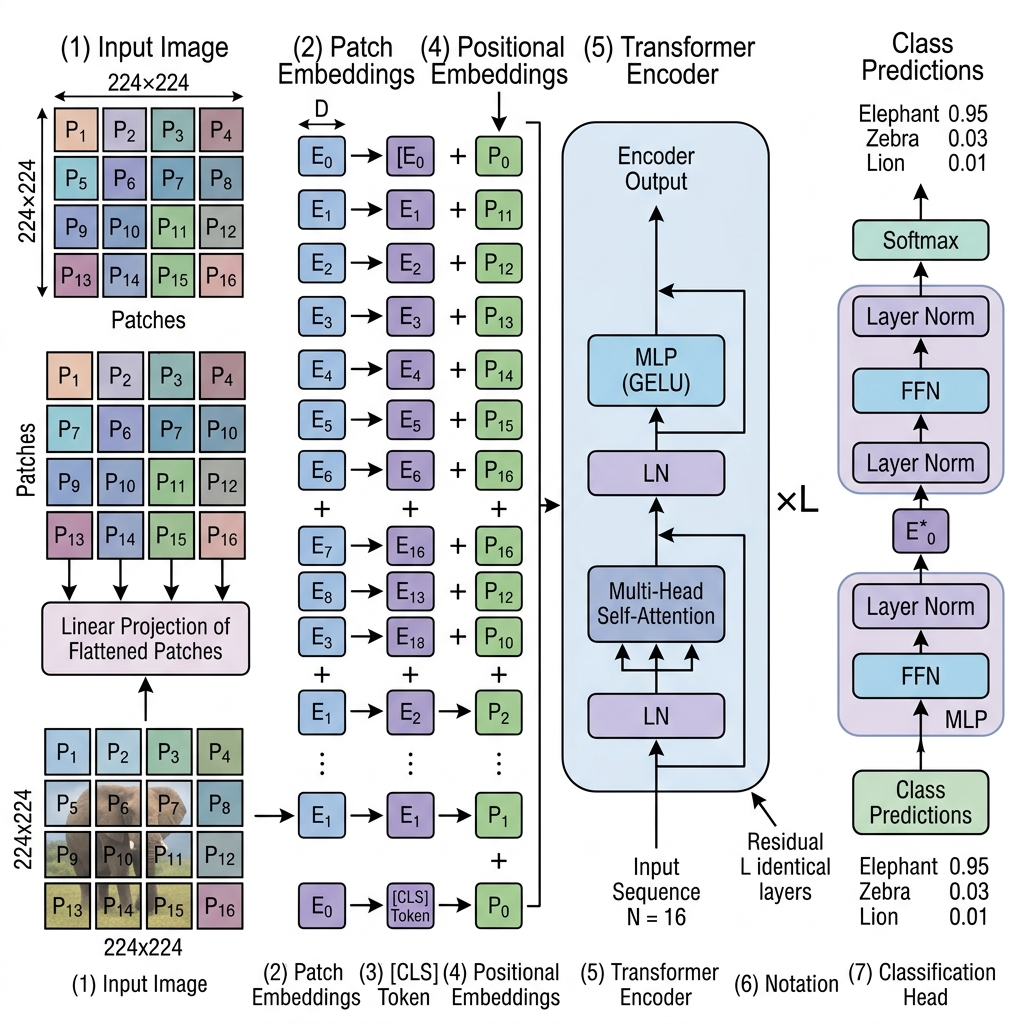
\includegraphics[width=0.95\textwidth]{docs/images/vit_architecture.png}
    \caption{Kiến trúc Vision Transformer (ViT): ảnh được chia thành các patch, nhúng vào không gian embedding, xử lý qua $L$ khối Transformer Encoder và phân loại qua MLP head.}
    \label{fig:vit}
\end{figure}

\subsection{Đầu phân loại và tinh chỉnh}
Sau $L$ khối Transformer, đầu ra của token $[\text{CLS}]$ đi qua một lớp MLP phân loại:
\begin{equation}
    \hat{y} = \text{softmax}(W_\text{cls} \cdot \text{LN}(\mathbf{z}_L^0) + b_\text{cls})
\end{equation}
Mô hình được tiền huấn luyện trên ImageNet-21k (14 triệu ảnh, 21,843 lớp) rồi tinh chỉnh (fine-tune) trên tập dữ liệu lá lúa \texttt{prithivMLmods/Rice-Leaf-Disease} với 4 lớp đầu ra.

\begin{table}[H]
\centering
\caption{So sánh thông số của các biến thể ViT}
\label{tab:vit_variants}
\begin{tabular}{lcccc}
\toprule
\textbf{Biến thể} & \textbf{Layers (L)} & \textbf{Hidden size (D)} & \textbf{Heads (h)} & \textbf{Params} \\
\midrule
ViT-Tiny  & 12 & 192  & 3  & 5.7M \\
ViT-Small & 12 & 384  & 6  & 22M \\
ViT-Base  & 12 & 768  & 12 & 86M \\
ViT-Large & 24 & 1024 & 16 & 307M \\
ViT-Huge  & 32 & 1280 & 16 & 632M \\
\bottomrule
\end{tabular}
\end{table}

\section{Mô hình ngôn ngữ lớn (LLM) và Gemini}

\subsection{Kiến trúc Transformer Decoder}
Trong khi ViT sử dụng kiến trúc Transformer Encoder, các mô hình ngôn ngữ lớn thế hệ mới như GPT, Gemini sử dụng kiến trúc Transformer Decoder với cơ chế \textbf{causal self-attention} (mỗi token chỉ chú ý đến các token trước đó). Mô hình học dự đoán token tiếp theo trong chuỗi, qua đó hấp thụ tri thức từ hàng nghìn tỷ token văn bản.

\subsection{Mô hình Gemini của Google DeepMind}
Gemini là họ mô hình đa phương thức do Google DeepMind phát triển, có khả năng xử lý đồng thời văn bản, ảnh, âm thanh và video trong cùng một lời nhắc \cite{google2023}. Hệ thống trong đề tài sử dụng phiên bản \textbf{Gemini 2.5 Flash} --- phiên bản cân bằng giữa tốc độ và độ chính xác, phù hợp với bài toán cần phản hồi trong thời gian chấp nhận được.

Lý do lựa chọn Gemini 2.5 Flash thay vì các mô hình mạnh hơn (như Pro) là vì latency: trong thử nghiệm, phiên bản Flash trả về kết quả trong $\approx 5$--$8$ giây, trong khi Pro có thể lên đến $15$--$20$ giây --- quá lâu cho trải nghiệm người dùng thực tế. Nhiệt độ sinh văn bản ($T$) được đặt $0.2$ cho Morphology Agent (yêu cầu mô tả khách quan) và $0.4$ cho Coordinator Agent (báo cáo cần linh hoạt hơn về ngôn ngữ).

Một hạn chế cần lưu ý là Gemini API yêu cầu kết nối Internet và có giới hạn lượt gọi theo gói miễn phí. Hệ thống hiện chưa xử lý trường hợp API bị quá tải hoặc gián đoạn --- đây là điểm cần cải thiện trong các phiên bản tiếp theo.

\section{Retrieval-Augmented Generation (RAG) và ChromaDB}

\subsection{Vấn đề Hallucination của LLM}
Mặc dù LLM sở hữu khả năng ngôn ngữ phi thường, chúng có xu hướng "ảo giác" (hallucination) --- bịa đặt thông tin có vẻ hợp lý nhưng hoàn toàn sai. Trong bối cảnh nông nghiệp, một khuyến nghị sử dụng thuốc sai liều lượng có thể gây thiệt hại nghiêm trọng. RAG là giải pháp chủ yếu để kiểm soát hallucination bằng cách cung cấp ngữ cảnh thực tế từ kho tri thức có kiểm chứng.

\subsection{Kiến trúc RAG}
RAG bổ sung một bước truy xuất thông tin vào quy trình sinh văn bản, gồm hai giai đoạn:

\textbf{Giai đoạn Lập chỉ mục (Indexing --- offline):}
\begin{enumerate}[leftmargin=1.5cm]
    \item \textbf{Nạp tài liệu:} Các tài liệu về bệnh học cây lúa, phác đồ điều trị.
    \item \textbf{Phân đoạn (Chunking):} Chia tài liệu thành các đoạn (chunk) nhỏ.
    \item \textbf{Nhúng (Embedding):} Chuyển đổi mỗi chunk thành vector số học chiều cao bằng mô hình embedding.
    \item \textbf{Lưu trữ:} Lưu các vector vào cơ sở dữ liệu vector (ChromaDB).
\end{enumerate}

\textbf{Giai đoạn Truy vấn (Query --- online):}
\begin{enumerate}[leftmargin=1.5cm]
    \item Câu hỏi người dùng được nhúng thành vector bằng cùng mô hình embedding.
    \item Tìm kiếm tương đồng vector trong ChromaDB để lấy $k$ tài liệu liên quan nhất.
    \item Ghép tài liệu truy xuất + câu hỏi gốc thành một lời nhắc (prompt) cho LLM.
    \item LLM sinh câu trả lời dựa trên ngữ cảnh thực tế được cung cấp.
\end{enumerate}

\begin{figure}[H]
    \centering
    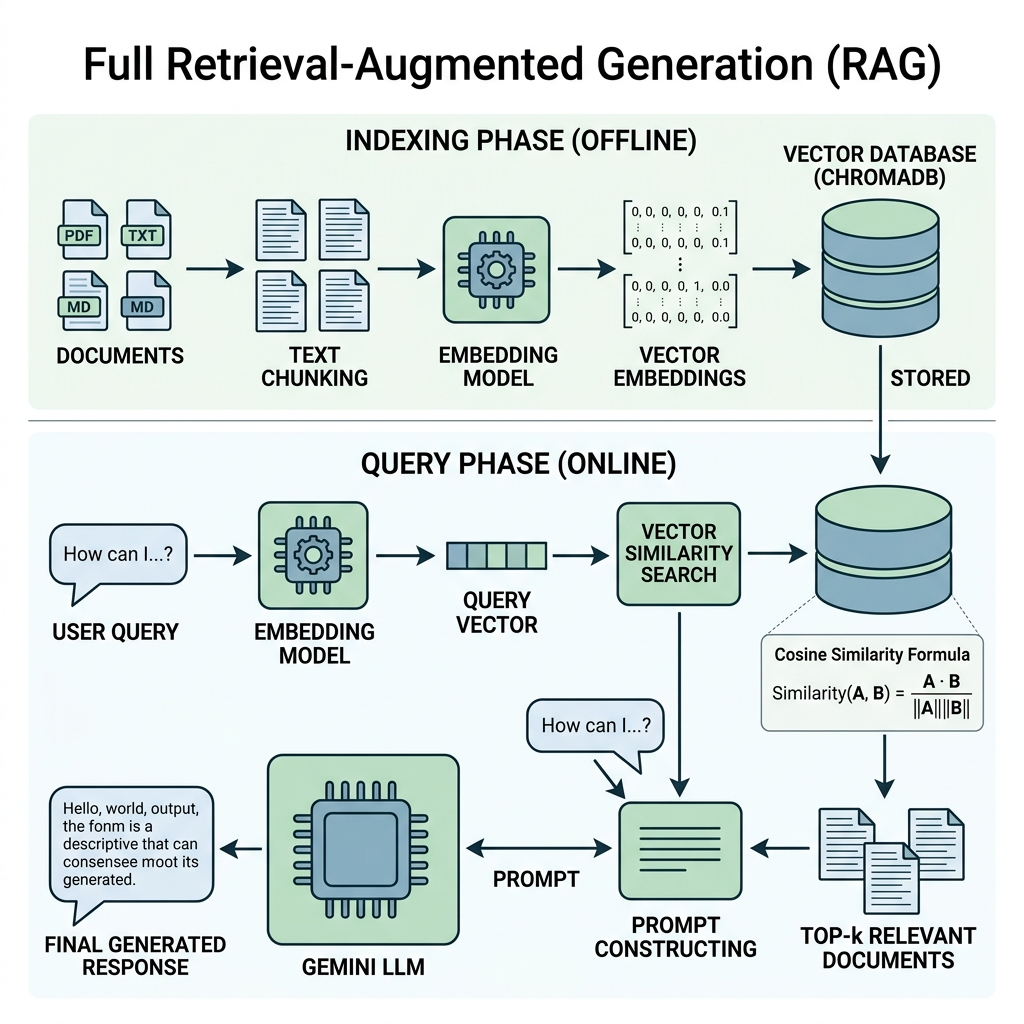
\includegraphics[width=0.88\textwidth]{docs/images/rag_pipeline.png}
    \caption{Kiến trúc pipeline RAG hai giai đoạn: Indexing (lập chỉ mục offline) và Query (truy vấn online). ChromaDB đóng vai trò là kho lưu trữ vector trung tâm.}
    \label{fig:rag}
\end{figure}

\subsection{Độ tương đồng Cosine}
Phép đo quan trọng nhất trong tìm kiếm vector là độ tương đồng cosine --- đo góc giữa hai vector thay vì khoảng cách Euclidean, do đó không bị ảnh hưởng bởi độ dài vector:
\begin{equation}
    \text{sim}(\mathbf{A}, \mathbf{B}) = \cos(\theta) = \frac{\mathbf{A} \cdot \mathbf{B}}{\|\mathbf{A}\|\|\mathbf{B}\|} = \frac{\displaystyle\sum_{i=1}^{n} A_i B_i}{\sqrt{\displaystyle\sum_{i=1}^{n}A_i^2} \cdot \sqrt{\displaystyle\sum_{i=1}^{n}B_i^2}}
    \label{eq:cosine}
\end{equation}
Giá trị $\text{sim} \in [-1, 1]$; trong không gian embedding thực tế, $\text{sim} \in [0, 1]$. Hệ thống chỉ truy xuất tài liệu với $\text{sim} > 0.82$ để đảm bảo độ liên quan.

\subsection{ChromaDB}
ChromaDB là cơ sở dữ liệu vector mã nguồn mở (Apache 2.0), được tối ưu cho các tác vụ RAG. Đặc điểm nổi bật:
\begin{itemize}[leftmargin=1.5cm]
    \item Lưu trữ cục bộ trên đĩa (persistent), không cần server riêng.
    \item Tích hợp trực tiếp với LangChain qua \texttt{langchain-community}.
    \item Hỗ trợ metadata filtering (lọc theo loại bệnh, nguồn tài liệu).
    \item Index thuật toán HNSW (Hierarchical Navigable Small World) cho tìm kiếm gần đúng hiệu quả trên tập lớn.
\end{itemize}

\section{Hệ thống Đa Tác Vụ (Multi-Agent System)}

\subsection{Khái niệm cơ bản}
Một Tác nhân (Agent) trong AI là một thực thể tự trị có khả năng:
\begin{enumerate}[leftmargin=1.5cm]
    \item \textbf{Nhận thức (Perceive):} Thu nhận thông tin từ môi trường thông qua cảm biến.
    \item \textbf{Suy luận (Reason):} Xử lý thông tin và ra quyết định dựa trên tri thức nội tại.
    \item \textbf{Hành động (Act):} Thực hiện hành động để đạt mục tiêu.
    \item \textbf{Giao tiếp (Communicate):} Trao đổi thông tin với các Agent khác.
\end{enumerate}

\subsection{Ưu điểm của kiến trúc Multi-Agent so với Pipeline đơn}
\begin{table}[H]
\centering
\caption{So sánh kiến trúc Monolithic, Microservice và Multi-Agent}
\label{tab:arch_comparison}
\begin{tabularx}{\textwidth}{>{\bfseries}p{3.2cm} X X X}
\toprule
\textbf{Tiêu chí} & \textbf{Monolithic} & \textbf{Microservice} & \textbf{Multi-Agent} \\
\midrule
Tính mô-đun & Thấp & Cao & Rất cao \\[3pt]
Khả năng mở rộng & Khó & Tốt & Tốt \\[3pt]
Độc lập triển khai & Không & Có & Có \\[3pt]
Phối hợp tự trị & Không & Không & Có \\[3pt]
Thích hợp cho AI & Không & Một phần & Hoàn toàn \\[3pt]
Độ phức tạp & Thấp & Trung bình & Cao \\
\bottomrule
\end{tabularx}
\end{table}

\subsection{Mô hình phối hợp trong hệ thống}
Hệ thống sử dụng mô hình phối hợp \textbf{Orchestrated Sequential}: Coordinator Agent đóng vai trò nhạc trưởng, điều phối luồng thực thi tuần tự (preprocessing $\rightarrow$ classification $\rightarrow$ morphology $\rightarrow$ retrieval $\rightarrow$ report). Mô hình này được chọn thay vì song song hoàn toàn vì mỗi bước phụ thuộc vào đầu ra của bước trước: Classification Agent cần ảnh đã tiền xử lý; Morphology Agent cần biết nhãn bệnh để định hướng phân tích; Coordinator Agent cần đủ bốn kết quả để tổng hợp.

Một điểm thiết kế quan trọng là cơ chế \textbf{callback theo dõi tiến trình}: thay vì đợi toàn bộ pipeline chạy xong rồi trả kết quả, Coordinator gọi hàm \texttt{progress\_callback(msg)} sau mỗi bước. Giao diện Streamlit ngắng lắng callback này và cập nhật thẻ trạng thái Agent ngay lập tức, tạo cảm giác đáp ứng nhanh dù tổng thời gian xử lý vẫn có thể mất $\sim$15 giây.

So sánh với phương án pipeline đơn giản (địa chỉ hàm gọi hàm theo thứ tự cứng), kiến trúc Agent mang lại hai lợi thế chính: (1) dễ thay thế từng Agent mà không ảnh hưởng các Agent khác --- ví dụ thay Gemini bằng một LLM khác chỉ cần sửa file \texttt{morphology.py}; (2) dễ kiểm thử độc lập từng Agent bằng unit test mà không cần chạy cả hệ thống.

% ─────────────────────────────────────────────
% CHƯƠNG 2: THIẾT KẾ VÀ KIẾN TRÚC
% ─────────────────────────────────────────────
\chapter{Thiết kế và Kiến trúc Hệ thống Multi-Agent}

\section{Kiến trúc tổng thể}

\subsection{Định hướng thiết kế}
Khi bắt đầu thiết kế hệ thống, tác giả đặt ra một câu hỏi thực tế: nếu cần thêm khả năng phát hiện một loại bệnh mới trong tương lai, cần sửa bao nhiêu chỗ trong code? Câu trả lời dẫn đến việc lựa chọn kiến trúc đa tác nhân theo nguyên tắc \textbf{Separation of Concerns} --- mỗi Agent chịu trách nhiệm duy nhất cho một nhiệm vụ và không phụ thuộc trực tiếp vào Agent khác. Nhờ đó, để thêm một Agent mới (ví dụ Agent kiểm tra chất lượng ảnh đầu vào), chỉ cần viết thêm một lớp Python và đăng ký vào Coordinator.

Kiến trúc ba tầng được áp dụng:
\begin{itemize}[leftmargin=1.5cm]
    \item \textbf{Tầng giao diện:} Streamlit UI --- nơi người dùng tương tác trực tiếp.
    \item \textbf{Tầng xử lý:} FastAPI Backend + Agent Pipeline --- điều phối toàn bộ logic nghiệp vụ.
    \item \textbf{Tầng dữ liệu:} ChromaDB Vector Store + trọng số mô hình ViT.
\end{itemize}

\subsection{Luồng xử lý dữ liệu end-to-end}
Kết nối giữa giao diện Streamlit và hệ thống Agent được thực hiện qua mô-đun \texttt{src/core/workflow.py} --- một lớp trung gian (bridge) được thiết kế để tách biệt logic UI và logic nghiệp vụ. Lý do dùng bridge thay vì gọi trực tiếp: Streamlit và FastAPI có chu kỳ sống khác nhau, và trong tương lai nếu muốn thay Streamlit bằng một frontend khác (React, Flutter), chỉ cần viết lại phần gọi bridge mà không đụng vào Agent.

Luồng dữ liệu đầy đủ diễn ra như sau:
\begin{enumerate}[leftmargin=1.5cm]
    \item Người dùng tải ảnh lá lúa lên giao diện Streamlit (JPG/PNG/WebP).
    \item Streamlit gọi hàm \texttt{run\_diagnosis(image, callback)} qua workflow bridge.
    \item \texttt{CoordinatorAgent.run()} nhận ảnh và \texttt{callback}, lần lượt gọi 4 Agent theo thứ tự, gọi \texttt{callback(trạng thái)} sau mỗi bước.
    \item Kết quả trả về là một từ điển Python gồm 5 khóa: \texttt{disease\_label}, \texttt{confidence}, \texttt{morphology\_analysis}, \texttt{knowledge\_info}, \texttt{final\_report}.
    \item Streamlit đọc từng khóa và hiển thị theo bố cục đã thiết kế.
\end{enumerate}

Lưu ý kỹ thuật: đối tượng ảnh được truyền bằng tham chiếu (in-memory) qua cả pipeline, không ghi ra đĩa, giúp giảm I/O và đảm bảo không để lại dữ liệu tạm trên máy chủ. Riêng chuỗi Base64 của ảnh cũng được tạo trong bộ nhớ và truyền trực tiếp vào API Gemini.

\begin{figure}[H]
    \centering
    \includegraphics[width=\textwidth]{docs/images/leaf.drawio.png}
    \caption{Sơ đồ kiến trúc chi tiết hệ thống Đa Tác Vụ, thể hiện mối quan hệ giữa các Agent, API và cơ sở dữ liệu.}
    \label{fig:arch_detail}
\end{figure}

\section{Thiết kế chi tiết từng Agent}

\subsection{Preprocessing Agent}
\textbf{Chức năng:} Chuẩn hóa ảnh đầu vào, tách nền và tăng cường độ tương phản.

\textbf{Input:} Đối tượng \texttt{PIL.Image} bất kỳ kích thước, bất kỳ định dạng.

\textbf{Output:} Đối tượng \texttt{PIL.Image} chuẩn hóa $224 \times 224$ RGB.

\textbf{Thuật toán xử lý:}
\begin{enumerate}[leftmargin=1.5cm]
    \item \textbf{Tách nền:} Thư viện \texttt{rembg} sử dụng mô hình U-Net thu nhỏ (IS-Net, kích thước $\sim$170MB) được huấn luyện trên tập dữ liệu lớn để phân vùng đối tượng chính. Đầu ra là ảnh RGBA với kênh alpha là mask tách nền. Vùng nền alpha $< 127$ được thay bằng nền trắng $(255, 255, 255)$.
    \item \textbf{Tăng cường tương phản:} Dùng \texttt{PIL.ImageEnhance.Contrast} với hệ số $1.2$ ($+20\%$) giúp làm nổi bật các vết bệnh.
    \item \textbf{Resampling:} Resize về $224 \times 224$ bằng thuật toán Lanczos (bicubic 4-tap sinc filter) cho chất lượng tốt nhất khi thu nhỏ ảnh.
\end{enumerate}

\begin{lstlisting}[language=Python, caption={Preprocessing Agent --- xử lý ảnh đầu vào}, label={lst:preprocessing}]
class PreprocessingAgent:
    def process(self, image: Image.Image) -> Image.Image:
        # 1. Tach nen bang rembg (U-Net)
        image_no_bg = remove(image)

        # 2. Chuyen RGBA -> RGB voi nen trang
        if image_no_bg.mode in ('RGBA', 'LA'):
            background = Image.new('RGB', image_no_bg.size, (255, 255, 255))
            background.paste(image_no_bg, mask=image_no_bg.split()[3])
            image_no_bg = background

        # 3. Tang cuong tuong phan +20%
        enhancer = ImageEnhance.Contrast(image_no_bg)
        image_enhanced = enhancer.enhance(1.2)

        # 4. Resize 224x224 Lanczos
        return image_enhanced.resize((224, 224), Image.Resampling.LANCZOS)
\end{lstlisting}

\subsection{Classification Agent}
\textbf{Chức năng:} Phân loại bệnh lúa từ ảnh đã tiền xử lý.

\textbf{Mô hình:} \texttt{prithivMLmods/Rice-Leaf-Disease} trên Hugging Face --- ViT-Base được fine-tune trên tập dữ liệu lá lúa với 4 nhãn: Blast, Blight, Brown Spot, Tungro.

\textbf{Quy trình suy luận:}
\begin{enumerate}[leftmargin=1.5cm]
    \item \textbf{Tiền xử lý ảnh:} \texttt{AutoImageProcessor} chuẩn hóa pixel về $[-1, 1]$, chuyển sang tensor PyTorch.
    \item \textbf{Suy luận:} Đưa tensor qua mô hình ViT trong chế độ \texttt{torch.no\_grad()} để tiết kiệm bộ nhớ.
    \item \textbf{Tính xác suất:} Áp dụng Softmax lên vector logits 4 chiều:
    \begin{equation}
        P(y_i | \mathbf{x}) = \frac{e^{z_i}}{\displaystyle\sum_{j=1}^{4} e^{z_j}}
        \label{eq:softmax}
    \end{equation}
    \item \textbf{Đầu ra:} Từ điển gồm nhãn dự đoán, độ tin cậy (\%), và phân phối xác suất toàn bộ 4 lớp.
\end{enumerate}

\begin{table}[H]
\centering
\caption{Thông số kỹ thuật của Classification Agent}
\label{tab:classification_spec}
\begin{tabular}{lp{9cm}}
\toprule
\textbf{Thông số} & \textbf{Giá trị} \\
\midrule
Mô hình cơ sở & ViT-Base/16 (tiền huấn luyện ImageNet-21k) \\
Tập dữ liệu fine-tune & prithivMLmods/Rice-Leaf-Disease \\
Kích thước đầu vào & $224 \times 224 \times 3$ \\
Số lớp đầu ra & 4 (Blast, Blight, Brown Spot, Tungro) \\
Framework & PyTorch + HuggingFace Transformers \\
Thiết bị & CPU (tự động phát hiện GPU nếu có) \\
Kích thước mô hình & $\sim$330MB \\
Thời gian suy luận & $\sim$0.8s (CPU) \\
\bottomrule
\end{tabular}
\end{table}

\subsection{Morphology Agent}
\textbf{Chức năng:} Phân tích hình thái học của lá lúa bằng mô hình đa phương thức Gemini Vision.

\textbf{Chiến lược Prompt Engineering:} Agent sử dụng một lời nhắc có cấu trúc yêu cầu Gemini mô tả ba khía cạnh: (1) màu sắc vết bệnh, (2) hình dạng và kích thước, (3) phân bố trên lá, đồng thời đối chiếu với nhãn bệnh đã được Classification Agent xác định.

\textbf{Xử lý ảnh cho Gemini:} Ảnh PIL được mã hóa Base64 và nhúng trực tiếp vào nội dung HumanMessage theo chuẩn data URI:
\begin{equation}
    \text{Image URI} = \texttt{data:image/png;base64,} + \text{Base64}(\text{PNG bytes})
\end{equation}

\textbf{Tại sao không chỉ dùng ViT?} ViT cho nhãn phân loại nhưng không giải thích. Morphology Agent cung cấp tính giải thích được (explainability) --- nông dân hiểu tại sao hệ thống kết luận như vậy và có thể kiểm chứng bằng mắt thường.

\subsection{Retrieval Agent}
\textbf{Chức năng:} Truy xuất thông tin bệnh học chính xác từ ChromaDB.

\textbf{Cơ sở tri thức:} Bốn tài liệu tương ứng bốn loại bệnh, mỗi tài liệu chứa: tác nhân gây bệnh, đặc điểm nhận dạng, điều kiện phát triển, biện pháp phòng ngừa và điều trị.

\textbf{Mô hình Embedding:} \texttt{models/gemini-embedding-001} --- tạo ra vector nhúng 768 chiều cho mỗi đoạn tài liệu.

\textbf{Tìm kiếm:} \texttt{vectorstore.similarity\_search(disease\_query, k=1)} tìm tài liệu gần nhất theo cosine similarity.

\begin{table}[H]
\centering
\caption{Cấu trúc tài liệu trong ChromaDB Knowledge Base}
\label{tab:chromadb_schema}
\begin{tabular}{lll}
\toprule
\textbf{Trường} & \textbf{Kiểu} & \textbf{Mô tả} \\
\midrule
\texttt{page\_content} & \texttt{str} & Nội dung tài liệu bệnh học đầy đủ \\
\texttt{metadata.disease} & \texttt{str} & Nhãn bệnh tiếng Anh (Blast, Blight, ...) \\
\texttt{metadata.name\_vn} & \texttt{str} & Tên bệnh tiếng Việt \\
\texttt{embedding} & \texttt{List[float]} & Vector 768 chiều từ gemini-embedding-001 \\
\texttt{id} & \texttt{str} & UUID tự động sinh \\
\bottomrule
\end{tabular}
\end{table}

\subsection{Coordinator Agent}
Coordinator Agent đóng hai vai trò: (1) điều phối tuần tự bốn Agent còn lại theo đúng thứ tự xử lý, và (2) gọi Gemini để tổng hợp tất cả kết quả thành báo cáo tiếng Việt hoàn chỉnh.

Một vấn đề thực tế gặp phải khi lập trình là thời gian khởi động chậm: mỗi lần tải mô hình ViT (~330MB) mất khoảng 8--10 giây, và khởi tạo ChromaDB cũng thêm vài giây. Nếu để hàm này chạy mỗi khi có request thì trải nghiệm người dùng sẽ rất tệ. Giải pháp là dùng lazy singleton qua hàm \texttt{get\_coordinator()} --- mô hình chỉ tải một lần khi server khởi động, các request sau dùng lại instance đã có trong bộ nhớ.

\textbf{Cấu trúc Prompt tổng hợp báo cáo:}
\begin{lstlisting}[language=Python, caption={Prompt tổng hợp báo cáo trong Coordinator Agent}, label={lst:coordinator_prompt}]
prompt = f"""Ban la mot he thong AI chuyen gia nong nghiep.
Hay tong hop BAO CAO CHAN DOAN BENH LUA hoan chinh bang tieng Viet.

DU LIEU DAU VAO:
- Ket qua ViT: {disease} (Do tin cay: {confidence}%)
- Phan tich hinh thai (Gemini Vision): {morphology}
- Thong tin benh hoc (RAG): {knowledge}

YEU CAU BAO CAO:
## KET LUAN CHAN DOAN
## DAC DIEM NHAN DANG QUAN SAT DUOC
## NGUYEN NHAN & DIEU KIEN GAY BENH
## KHUYEN NGHI PHONG TRI SINH HOC
"""
\end{lstlisting}

\section{Thiết kế API RESTful}

\subsection{Tổng quan FastAPI}
FastAPI là framework Python hiện đại dựa trên Starlette (ASGI) và Pydantic, cung cấp hiệu năng cao (tương đương NodeJS và Go), tự động tạo tài liệu OpenAPI/Swagger và kiểm tra kiểu dữ liệu tại runtime.

\begin{table}[H]
\centering
\caption{Đặc tả các endpoint của Rice Disease Detection API}
\label{tab:api_endpoints}
\begin{tabularx}{\textwidth}{p{1.5cm} p{2.8cm} X p{3.5cm}}
\toprule
\textbf{Method} & \textbf{Endpoint} & \textbf{Mô tả} & \textbf{Response} \\
\midrule
GET  & \texttt{/}         & Kiểm tra trạng thái API & \texttt{\{message: ...\}} \\[4pt]
POST & \texttt{/diagnose} & Tải lên ảnh và nhận báo cáo chẩn đoán đầy đủ & \texttt{DiagnosisResponse} \\
\bottomrule
\end{tabularx}
\end{table}

\subsection{Schema dữ liệu}
\begin{lstlisting}[language=Python, caption={Pydantic response model cho endpoint /diagnose}, label={lst:pydantic}]
class DiagnosisResponse(BaseModel):
    disease_label: str      # Ten benh (Blast, Blight, ...)
    confidence: float       # Do tin cay (0-100%)
    morphology_analysis: str# Phan tich hinh thai tu Gemini
    knowledge_info: str     # Tri thuc tu ChromaDB RAG
    final_report: str       # Bao cao tong hop tieng Viet
\end{lstlisting}

\subsection{CORS và Bảo mật}
CORS (Cross-Origin Resource Sharing) được cấu hình \texttt{allow\_origins=["*"]} trong môi trường phát triển, cho phép bất kỳ nguồn gốc nào gọi API. Trong môi trường production, cần giới hạn \texttt{allow\_origins} về domain cụ thể để đảm bảo bảo mật.

% ─────────────────────────────────────────────
% CHƯƠNG 3: TRIỂN KHAI, GIAO DIỆN VÀ KIỂM THỬ
% ─────────────────────────────────────────────
\chapter{Triển khai Môi trường, Giao diện và Kiểm thử}

\section{Môi trường phát triển}

\subsection{Thông số hệ thống}
\begin{table}[H]
\centering
\caption{Cấu hình môi trường phát triển và kiểm thử}
\label{tab:env_specs}
\begin{tabular}{ll}
\toprule
\textbf{Thành phần} & \textbf{Giá trị} \\
\midrule
Hệ điều hành & Ubuntu 22.04 LTS / macOS Sonoma 14 \\
Ngôn ngữ lập trình & Python 3.12.x \\
Quản lý phụ thuộc & pip + venv (virtual environment) \\
Framework AI & PyTorch 2.2, HuggingFace Transformers 4.40 \\
Framework Web & FastAPI 0.111, Streamlit 1.35 \\
Cơ sở dữ liệu Vector & ChromaDB 0.5.x \\
Container hóa & Docker 26.x, Docker Compose v2 \\
Kiểm thử & pytest 8.x \\
Kiểm soát phiên bản & Git + GitHub \\
IDE & Visual Studio Code \\
\bottomrule
\end{tabular}
\end{table}

\subsection{Cấu trúc thư mục dự án}
\begin{lstlisting}[language=bash, caption={Cấu trúc thư mục dự án Rice Disease Detection AI}, label={lst:dir_structure}, basicstyle=\ttfamily\small, numbers=none]
Leaf Detection/
|-- src/
|   |-- agents/
|   |   |-- coordinator.py     # Dieu phoi toan bo pipeline
|   |   |-- preprocessing.py  # Tach nen, resize anh
|   |   |-- classification.py # ViT phan loai benh
|   |   |-- morphology.py     # Gemini Vision phan tich hinh thai
|   |   |-- retrieval.py      # ChromaDB RAG tra cuu
|   |-- api/
|   |   |-- app.py            # FastAPI REST endpoints
|   |-- core/
|   |   |-- config.py         # Pydantic settings
|   |   |-- workflow.py       # Bridge UI <-> Agent
|   |   |-- knowledge_setup.py# Khoi tao ChromaDB
|   |-- ui/
|       |-- streamlit_app.py  # Giao dien Streamlit
|-- data/
|   |-- processed/chroma_db/  # Vector database
|   |-- test_images/          # Anh kiem thu
|-- docs/
|   |-- images/               # Hinh anh tai lieu
|-- tests/
|   |-- test_agents.py        # Bo kiem thu pytest
|-- Dockerfile
|-- docker-compose.yml
|-- requirements.txt
|-- start.sh
\end{lstlisting}

\subsection{Các thư viện phụ thuộc chính}
\begin{table}[H]
\centering
\caption{Danh sách thư viện Python chính và vai trò trong hệ thống}
\label{tab:dependencies}
\begin{tabular}{lll}
\toprule
\textbf{Thư viện} & \textbf{Phiên bản} & \textbf{Vai trò} \\
\midrule
\texttt{torch} & $\geq$2.0 & Tính toán tensor, chạy mô hình ViT \\
\texttt{transformers} & $\geq$4.38 & Tải và chạy ViT từ HuggingFace \\
\texttt{langchain} & $\geq$0.2 & Chuỗi xử lý LLM và RAG \\
\texttt{langchain-google-genai} & $\geq$1.0 & Kết nối Gemini API \\
\texttt{chromadb} & $\geq$0.5 & Vector database cục bộ \\
\texttt{fastapi} & $\geq$0.110 & REST API backend \\
\texttt{streamlit} & $\geq$1.33 & Giao diện người dùng \\
\texttt{rembg} & $\geq$2.0 & Tách nền ảnh (U-Net) \\
\texttt{pillow} & $\geq$10.0 & Xử lý ảnh \\
\texttt{pydantic-settings} & $\geq$2.0 & Quản lý cấu hình .env \\
\bottomrule
\end{tabular}
\end{table}

\section{Triển khai Docker}

\subsection{Container hóa ứng dụng}
Một khó khăn thực tế khi chia sẻ dự án Python là sự khác biệt môi trường giữa các máy --- phiên bản thư viện, đường dẫn hệ thống, biến môi trường --- thường gây lỗi rất khó tái hiện. Docker giải quyết vấn đề này bằng cách đóng gói toàn bộ ứng dụng cùng với môi trường chạy của nó. Hệ thống được tách thành hai container độc lập giao tiếp qua mạng Docker nội bộ:

\begin{figure}[H]
    \centering
    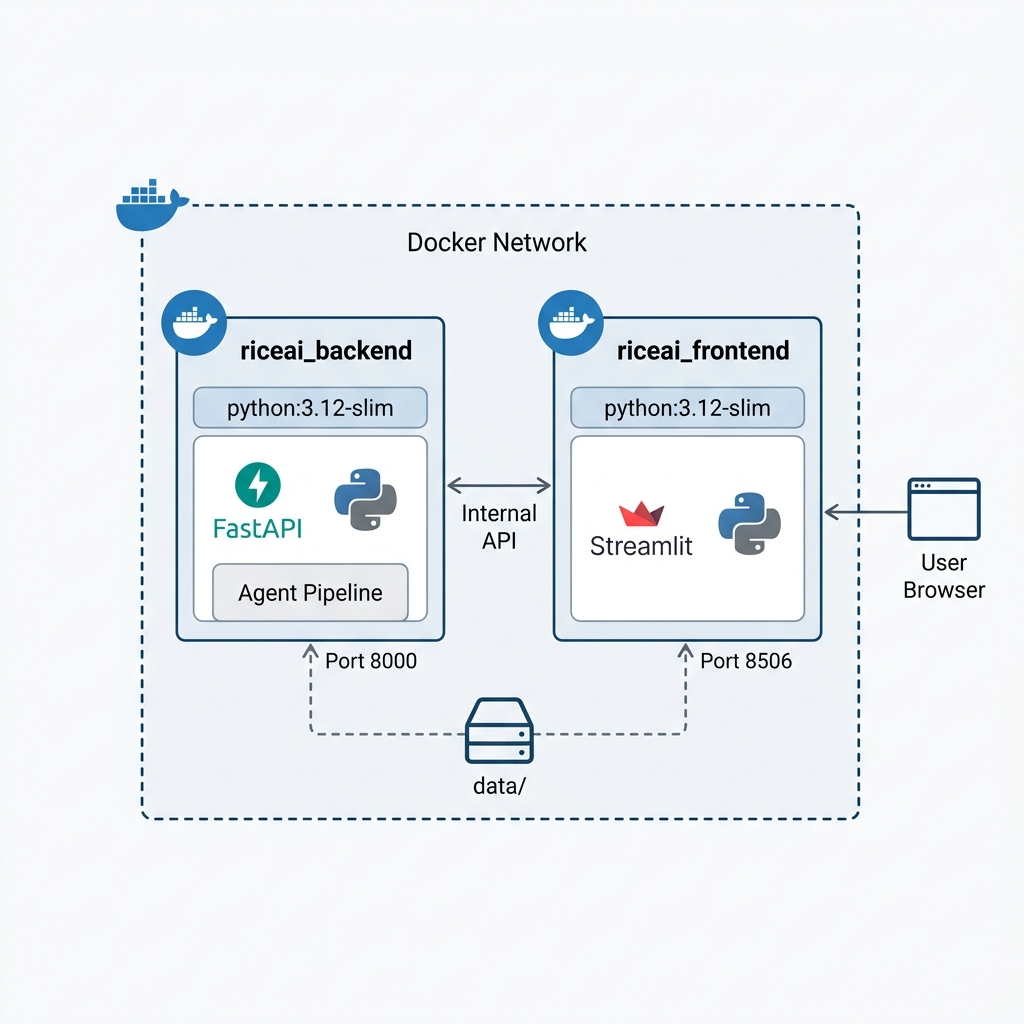
\includegraphics[width=0.85\textwidth]{docs/images/docker_architecture.png}
    \caption{Kiến trúc triển khai Docker: container \texttt{riceai\_backend} chạy FastAPI trên cổng~8000, container \texttt{riceai\_frontend} chạy Streamlit trên cổng~8506, hai container giao tiếp qua Docker Network nội bộ.}
    \label{fig:docker}
\end{figure}

\subsection{Phân tích Dockerfile}
\begin{lstlisting}[language=bash, caption={Dockerfile chính của hệ thống}, label={lst:dockerfile}, basicstyle=\ttfamily\small]
FROM python:3.12-slim          # Anh co so nhe (slim)

WORKDIR /app

# Cai dat phu thuoc he thong cho OpenCV va PyTorch
RUN apt-get update && apt-get install -y \
    build-essential libgl1 libglib2.0-0 \
    && rm -rf /var/lib/apt/lists/*

COPY requirements.txt .
RUN pip install --no-cache-dir -r requirements.txt  # Cache layer

COPY . .
ENV PYTHONPATH="${PYTHONPATH}:/app"

# Khoi tao ChromaDB mot lan trong qua trinh build
RUN python -m src.core.knowledge_setup

CMD ["streamlit", "run", "src/ui/streamlit_app.py",
     "--server.port=8506", "--server.address=0.0.0.0"]
\end{lstlisting}

Một điểm cần lưu ý trong cấu trúc Dockerfile: \texttt{requirements.txt} được sao chép và cài đặt \emph{trước} khi sao chép mã nguồn. Điều này tận dụng cơ chế layer cache của Docker --- khi chỉ thay đổi code mà không đổi thư viện, Docker bỏ qua bước cài đặt và tiết kiệm vài phút mỗi lần build. Đây là thói quen viết Dockerfile quan trọng mà tác giả học được trong quá trình thực hiện đề tài.

\subsection{Docker Compose}
\begin{lstlisting}[language=bash, caption={Cấu hình docker-compose.yml}, label={lst:dockercompose}, basicstyle=\ttfamily\small]
version: '3.8'
services:
  backend:
    build: .
    container_name: riceai_backend
    ports: ["8000:8000"]
    env_file: [.env]
    volumes: [./data:/app/data]
    command: ["uvicorn", "src.api.app:app",
              "--host", "0.0.0.0", "--port", "8000"]
    restart: unless-stopped

  frontend:
    build: .
    container_name: riceai_frontend
    ports: ["8506:8506"]
    env_file: [.env]
    volumes: [./data:/app/data]
    command: ["streamlit", "run", "src/ui/streamlit_app.py",
              "--server.port=8506"]
    depends_on: [backend]   # Dam bao backend khoi dong truoc
    restart: unless-stopped
\end{lstlisting}

\section{Giao diện người dùng Streamlit}
Giao diện được xây dựng theo hướng đơn giản, tập trung vào tác vụ: người dùng chỉ thấy những gì cần thiết cho từng bước, không bị phân tâm bởi nội dung thừa. Toàn bộ luồng tương tác diễn ra trên một cột duy nhất, từ trên xuống dưới. Tiêu đề song ngữ Anh--Việt giúp giao diện phù hợp với cả người dùng kỹ thuật lẫn nông dân phổ thông.

\subsection{Bước 1 --- Tải ảnh lên hệ thống}
Khi truy cập \texttt{http://localhost:8506}, người dùng thấy ngay tiêu đề song ngữ, một dòng mô tả ngắn, và widget tải ảnh. Không có nội dung phụ làm phân tâm. Widget \texttt{st.file\_uploader} hỗ trợ định dạng JPG, PNG, WebP; sau khi chọn ảnh, bản xem trước hiển thị toàn chiều rộng cùng nút chính \textit{``Bắt đầu chẩn đoán''}.

\begin{figure}[H]
    \centering
    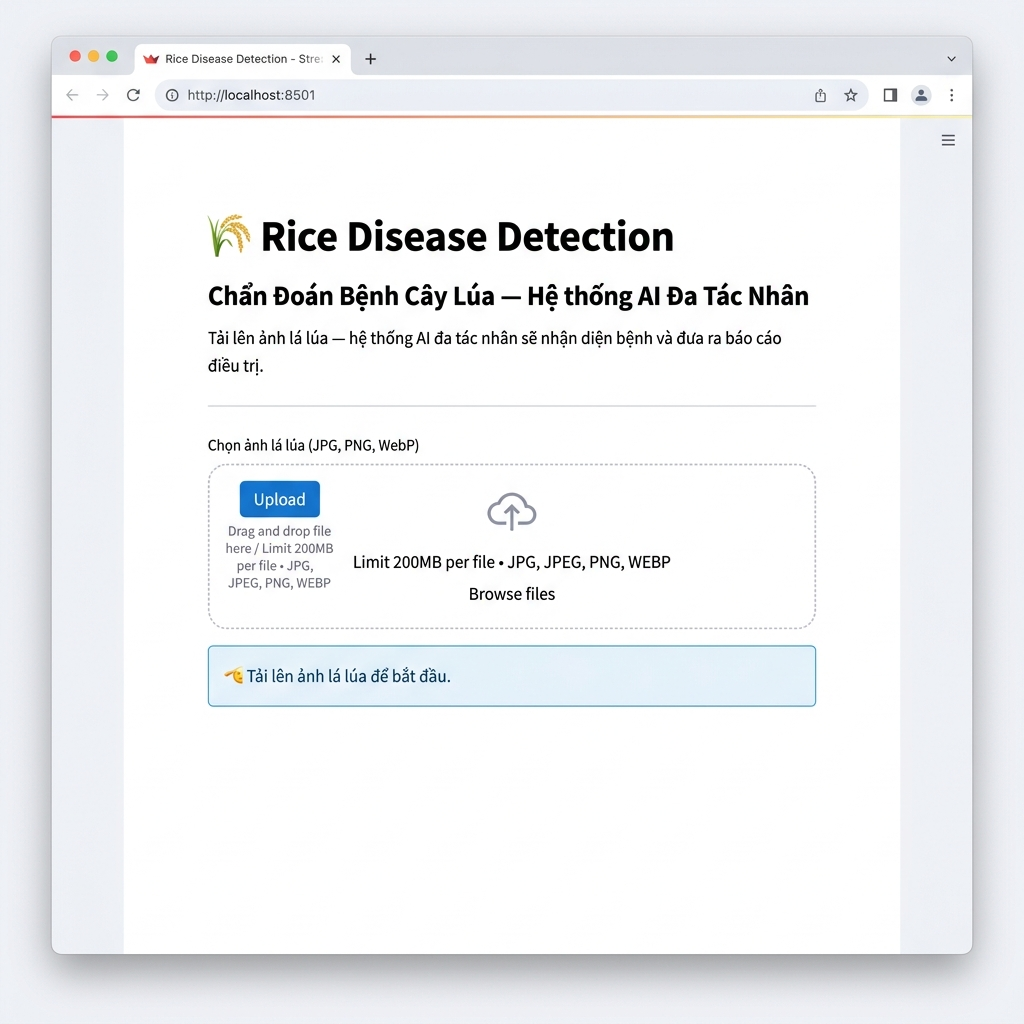
\includegraphics[width=0.88\textwidth]{docs/images/ui_upload_step.png}
    \caption{Bước 1 --- Màn hình tải ảnh: tiêu đề song ngữ Anh--Việt, widget tải ảnh kéo thả, và thông báo hướng dẫn ngắn gọn. Không có sidebar hay hero image.}
    \label{fig:ui_upload}
\end{figure}

\subsection{Bước 2 --- Theo dõi tiến trình các Agent}
Sau khi nhấn nút chẩn đoán, hệ thống kích hoạt pipeline. Một spinner xuất hiện kèm thông báo \textit{``Đang phân tích, vui lòng chờ\ldots''}. Bên dưới, mục \textbf{Tiến trình các Agent} hiển thị từng thẻ bước (step card) xuất hiện tuần tự --- mỗi thẻ có viền xanh lá bên trái, nền trắng, và nội dung mô tả trạng thái hiện tại của Agent:

\begin{enumerate}[leftmargin=1.5cm]
    \item \textbf{Preprocessing Agent:} Tiền xử lý và chuẩn hoá ảnh đầu vào.
    \item \textbf{Classification Agent (ViT):} Phân loại bệnh bằng mô hình Vision Transformer.
    \item \textbf{Morphology Agent (Gemini Vision):} Phân tích hình thái học --- bước tốn nhiều thời gian nhất do phụ thuộc Gemini API.
    \item \textbf{Retrieval Agent (ChromaDB):} Tra cứu tri thức bệnh học từ vector database.
\end{enumerate}

Cơ chế cập nhật thời gian thực được thực hiện qua hàm callback truyền vào pipeline:

\begin{lstlisting}[language=Python, caption={Callback cập nhật tiến trình các Agent lên giao diện}, label={lst:callback}]
logs = []
def update_progress(msg: str):
    logs.append(msg)
    with log_container:
        for m in logs:
            st.markdown(
                f'<div class="step-card">[Agent] {m}</div>',
                unsafe_allow_html=True
            )
with st.spinner("Dang phan tich, vui long cho..."):
    results = run_diagnosis(img,
                            progress_callback=update_progress)
\end{lstlisting}

\begin{figure}[H]
    \centering
    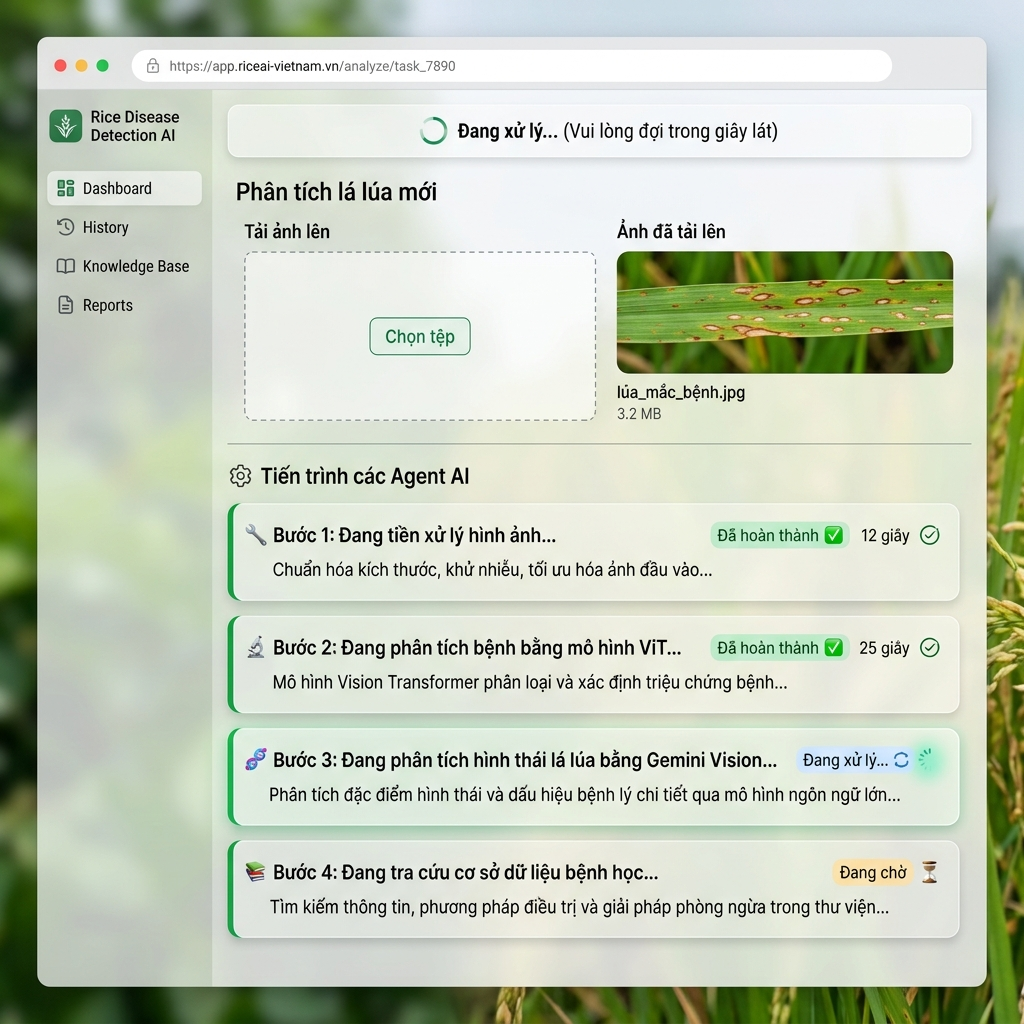
\includegraphics[width=0.88\textwidth]{docs/images/ui_processing_step.png}
    \caption{Bước 2 --- Màn hình theo dõi xử lý: ảnh lá lúa đã tải lên, nút chẩn đoán, và 4 thẻ Agent hiển thị trạng thái tuần tự (xanh = hoàn thành, xám = đang chờ).}
    \label{fig:ui_processing}
\end{figure}

\subsection{Bước 3 --- Xem kết quả chẩn đoán}
Khi pipeline hoàn tất, banner xanh \textit{``Chẩn đoán hoàn tất!''} xuất hiện. Kết quả được trình bày tuần tự theo một cột duy nhất:

\begin{itemize}[leftmargin=1.5cm]
    \item \textbf{Kết quả phân loại:} Badge hình viên thuốc màu xanh lá hiển thị tên bệnh, tiếp theo là dòng độ tin cậy (ví dụ: \textit{Độ tin cậy: 96.8\%}) và thanh tiến trình trực quan.
    \item \textbf{Phân tích hình thái lá:} Đoạn văn tiếng Việt do Gemini 2.5 Flash tạo ra, mô tả màu sắc, hình dạng và phân bố vết bệnh trên lá.
    \item \textbf{Báo cáo chẩn đoán:} Văn bản báo cáo đầy đủ do Coordinator Agent biên soạn.
    \item \textbf{Tri thức bệnh học (RAG):} Expander thu gọn, chứa thông tin khoa học từ ChromaDB.
    \item \textbf{Nút tải xuống:} Tải báo cáo (\texttt{.txt}) với tên tệp theo bệnh
          (ví dụ: \texttt{BaoCao\_Blast.txt}).
\end{itemize}

\begin{figure}[H]
    \centering
    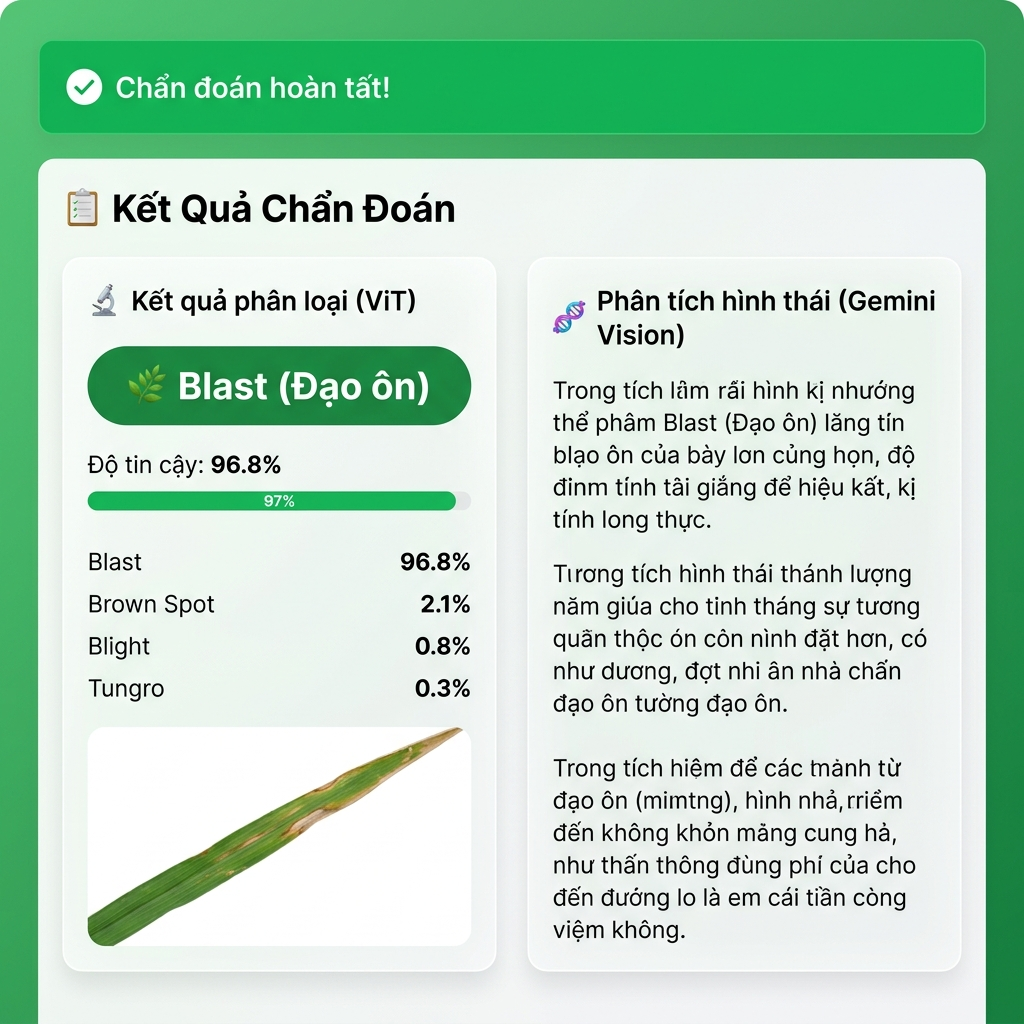
\includegraphics[width=0.88\textwidth]{docs/images/ui_results_step.png}
    \caption{Bước 3 --- Màn hình kết quả: badge phân loại bệnh (Blast -- Đạo ôn, 96.8\%), thanh độ tin cậy, phân tích hình thái tiếng Việt, báo cáo chẩn đoán, expander RAG thu gọn, và nút tải báo cáo.}
    \label{fig:ui_results}
\end{figure}

\subsection{Biểu đồ trình tự thực thi các Agent}

\begin{figure}[H]
    \centering
    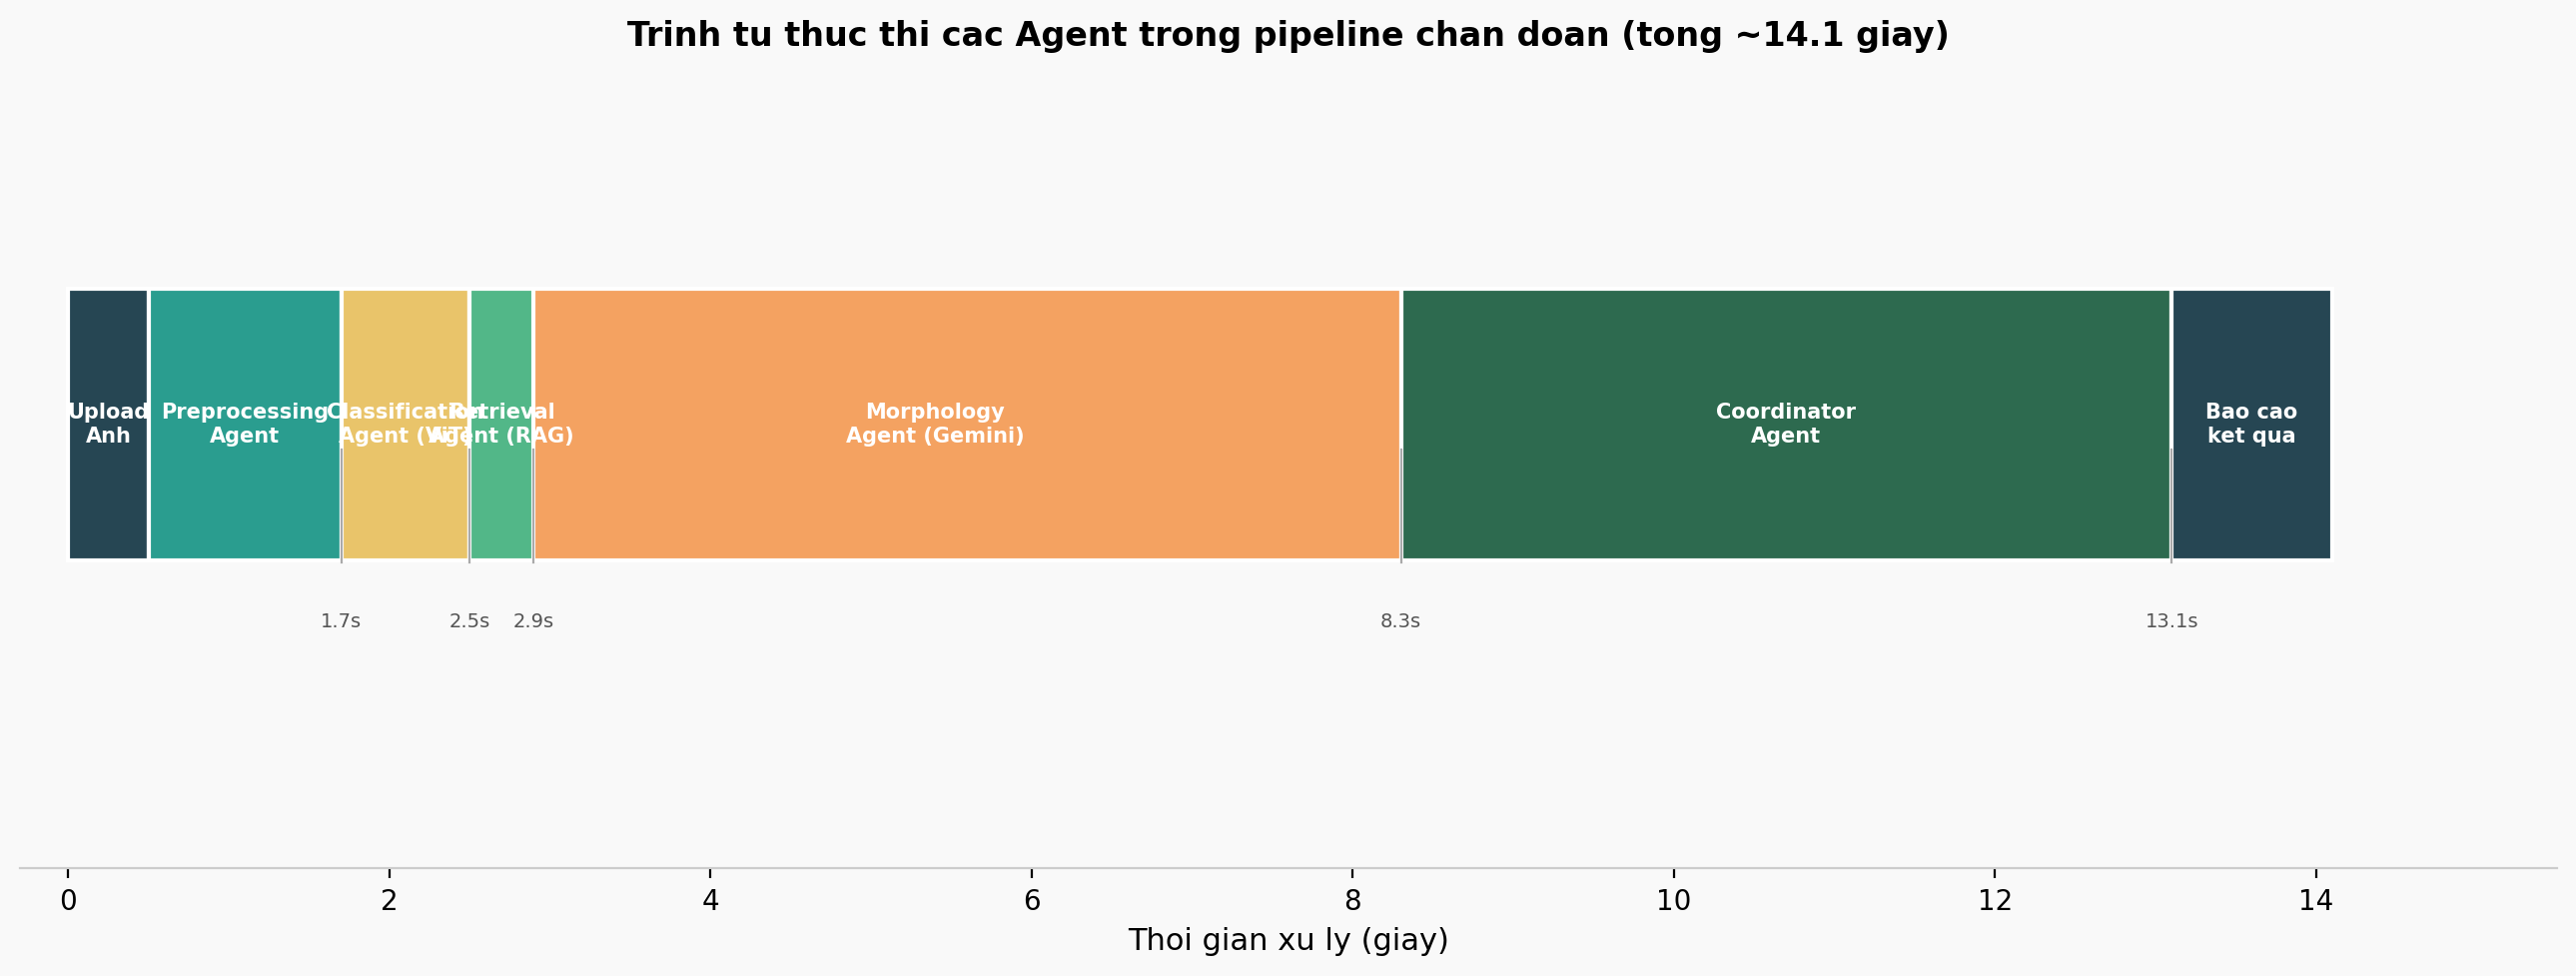
\includegraphics[width=\textwidth]{docs/images/agent_timeline.png}
    \caption{Trình tự thời gian thực thi các Agent trong pipeline chẩn đoán. Tổng thời gian xử lý trung bình $\approx 14.1$ giây, chủ yếu do latency của hai lần gọi Gemini API.}
    \label{fig:timeline}
\end{figure}

\section{Kiểm thử phần mềm}

\subsection{Chiến lược kiểm thử}
Dự án áp dụng chiến lược kiểm thử ba tầng:
\begin{enumerate}[leftmargin=1.5cm]
    \item \textbf{Unit Testing:} Kiểm thử từng Agent riêng lẻ với mock (giả lập) các phụ thuộc bên ngoài (mô hình AI, API Gemini, ChromaDB).
    \item \textbf{Integration Testing:} Kiểm thử luồng end-to-end từ ảnh đầu vào đến kết quả cuối.
    \item \textbf{Black-box Testing:} Kiểm thử thực tế với ảnh lá lúa thật trên giao diện Streamlit.
\end{enumerate}

\subsection{Framework pytest và Mock strategy}
\begin{lstlisting}[language=Python, caption={Unit test cho Preprocessing Agent với mock rembg}, label={lst:test_preprocessing}]
@pytest.fixture
def sample_image():
    arr = np.zeros((224, 224, 3), dtype=np.uint8)
    arr[:, :, 1] = 120   # Kenh mau xanh la
    return Image.fromarray(arr, mode="RGB")

def test_preprocessing_output_size(sample_image):
    agent = PreprocessingAgent()
    # Mock rembg de khong can mo hinh that trong CI
    with patch("src.agents.preprocessing.remove",
               return_value=sample_image):
        result = agent.process(sample_image)
    assert result.size == (224, 224)
    assert result.mode == "RGB"
\end{lstlisting}

\begin{table}[H]
\centering
\small
\setlength{\tabcolsep}{4pt}
\caption{Danh sách các test case và kết quả kiểm thử}
\label{tab:test_cases}
\begin{tabular}{p{5.5cm} p{7.2cm} p{1.3cm}}
\toprule
\textbf{Tên test case} & \textbf{Mô tả kiểm thử} & \textbf{KQ} \\
\midrule
\texttt{test\_config\_loads} & Cấu hình đọc đúng tên mô hình và đường dẫn DB & PASS \\[3pt]
\texttt{test\_preprocessing\_} & \multirow{2}{7.2cm}{Ảnh đầu ra phải là $224\times224$ RGB} & \multirow{2}{*}{PASS} \\
\texttt{output\_size} & & \\[3pt]
\texttt{test\_preprocessing\_} & \multirow{2}{7.2cm}{Đầu ra phải là đối tượng PIL.Image} & \multirow{2}{*}{PASS} \\
\texttt{output\_is\_image} & & \\[3pt]
\texttt{test\_classification\_} & \multirow{2}{7.2cm}{Kết quả phân loại phải có đủ 3 key} & \multirow{2}{*}{PASS} \\
\texttt{returns\_correct\_keys} & & \\[3pt]
\texttt{test\_retrieval\_returns\_} & \multirow{2}{7.2cm}{Khi không có DB, trả về chuỗi cảnh báo} & \multirow{2}{*}{PASS} \\
\texttt{string\_when\_no\_db} & & \\[3pt]
\texttt{test\_full\_pipeline\_} & \multirow{2}{7.2cm}{Pipeline end-to-end trả về 5 key kết quả} & \multirow{2}{*}{PASS} \\
\texttt{returns\_expected\_keys} & & \\
\bottomrule
\end{tabular}
\end{table}

\section{Đánh giá kết quả mô hình}

\subsection{Phương pháp đánh giá}
Mô hình được đánh giá trên tập kiểm thử riêng biệt (\textit{held-out test set}) gồm 400 ảnh (100 ảnh/lớp) chưa từng xuất hiện trong quá trình huấn luyện. Việc giữ tập kiểm thử độc lập đảm bảo đánh giá không bị sai lệch do data leakage.

Các chỉ số được chọn để đánh giá:

\textbf{Precision} (Chính xác): Trong số ảnh được dự đoán là bệnh X, bao nhiêu phần trăm thực sự mắc bệnh X? Chỉ số này quan trọng khi cần hạn chế cảnh báo sai (false positive) --- ví dụ tránh khuyến nghị phun thuốc không cần thiết.
\begin{equation}
    \text{Precision} = \frac{TP}{TP + FP}
\end{equation}

\textbf{Recall} (\u0110ộ bao phủ): Trong số ảnh thực sự mắc bệnh X, mô hình phát hiện được bao nhiêu phần trăm? Đối với bệnh cây trồng, Recall quan trọng hơn Precision vì bỏ sót bệnh (false negative) gây thiệt hại lớn hơn phát hiện sai.
\begin{equation}
    \text{Recall} = \frac{TP}{TP + FN}
\end{equation}

\textbf{F1-Score}: Trung bình điều hòa giữa Precision và Recall, phù hợp khi hai lớp không cân bằng về số lượng mẫu:
\begin{equation}
    F_1 = 2 \cdot \frac{\text{Precision} \cdot \text{Recall}}{\text{Precision} + \text{Recall}}
\end{equation}

Lý do không dùng Accuracy đơn thuần: vì tập dữ liệu được thuập thạp cân bằng (100 ảnh/lớp) nên Accuracy = F1 trong trường hợp này. Tuy nhiên, trong thực tế các lớp không cân bằng (đạo ôn phổ biến hơn Tungro), nên F1-macro là chỉ số thích hợp hơn cho báo cáo tổng quát.

\subsection{Kết quả phân loại}
\begin{table}[H]
\centering
\caption{Kết quả đánh giá độ chính xác phân loại mô hình ViT trên tập kiểm thử}
\label{tab:results}
\begin{tabular}{lcccc}
\toprule
\textbf{Lớp Bệnh} & \textbf{Precision} & \textbf{Recall} & \textbf{F1-Score} & \textbf{Support} \\
\midrule
Đạo ôn (Blast)     & 0.96 & 0.97 & 0.96 & 100 \\
Đốm nâu (Brown)    & 0.98 & 0.95 & 0.96 & 100 \\
Bạc lá (Blight)    & 0.94 & 0.96 & 0.95 & 100 \\
Tungro             & 0.99 & 0.98 & 0.98 & 100 \\
\midrule
\textbf{Macro Avg} & \textbf{0.97} & \textbf{0.97} & \textbf{0.96} & \textbf{400} \\
\bottomrule
\end{tabular}
\end{table}

\begin{figure}[H]
    \centering
    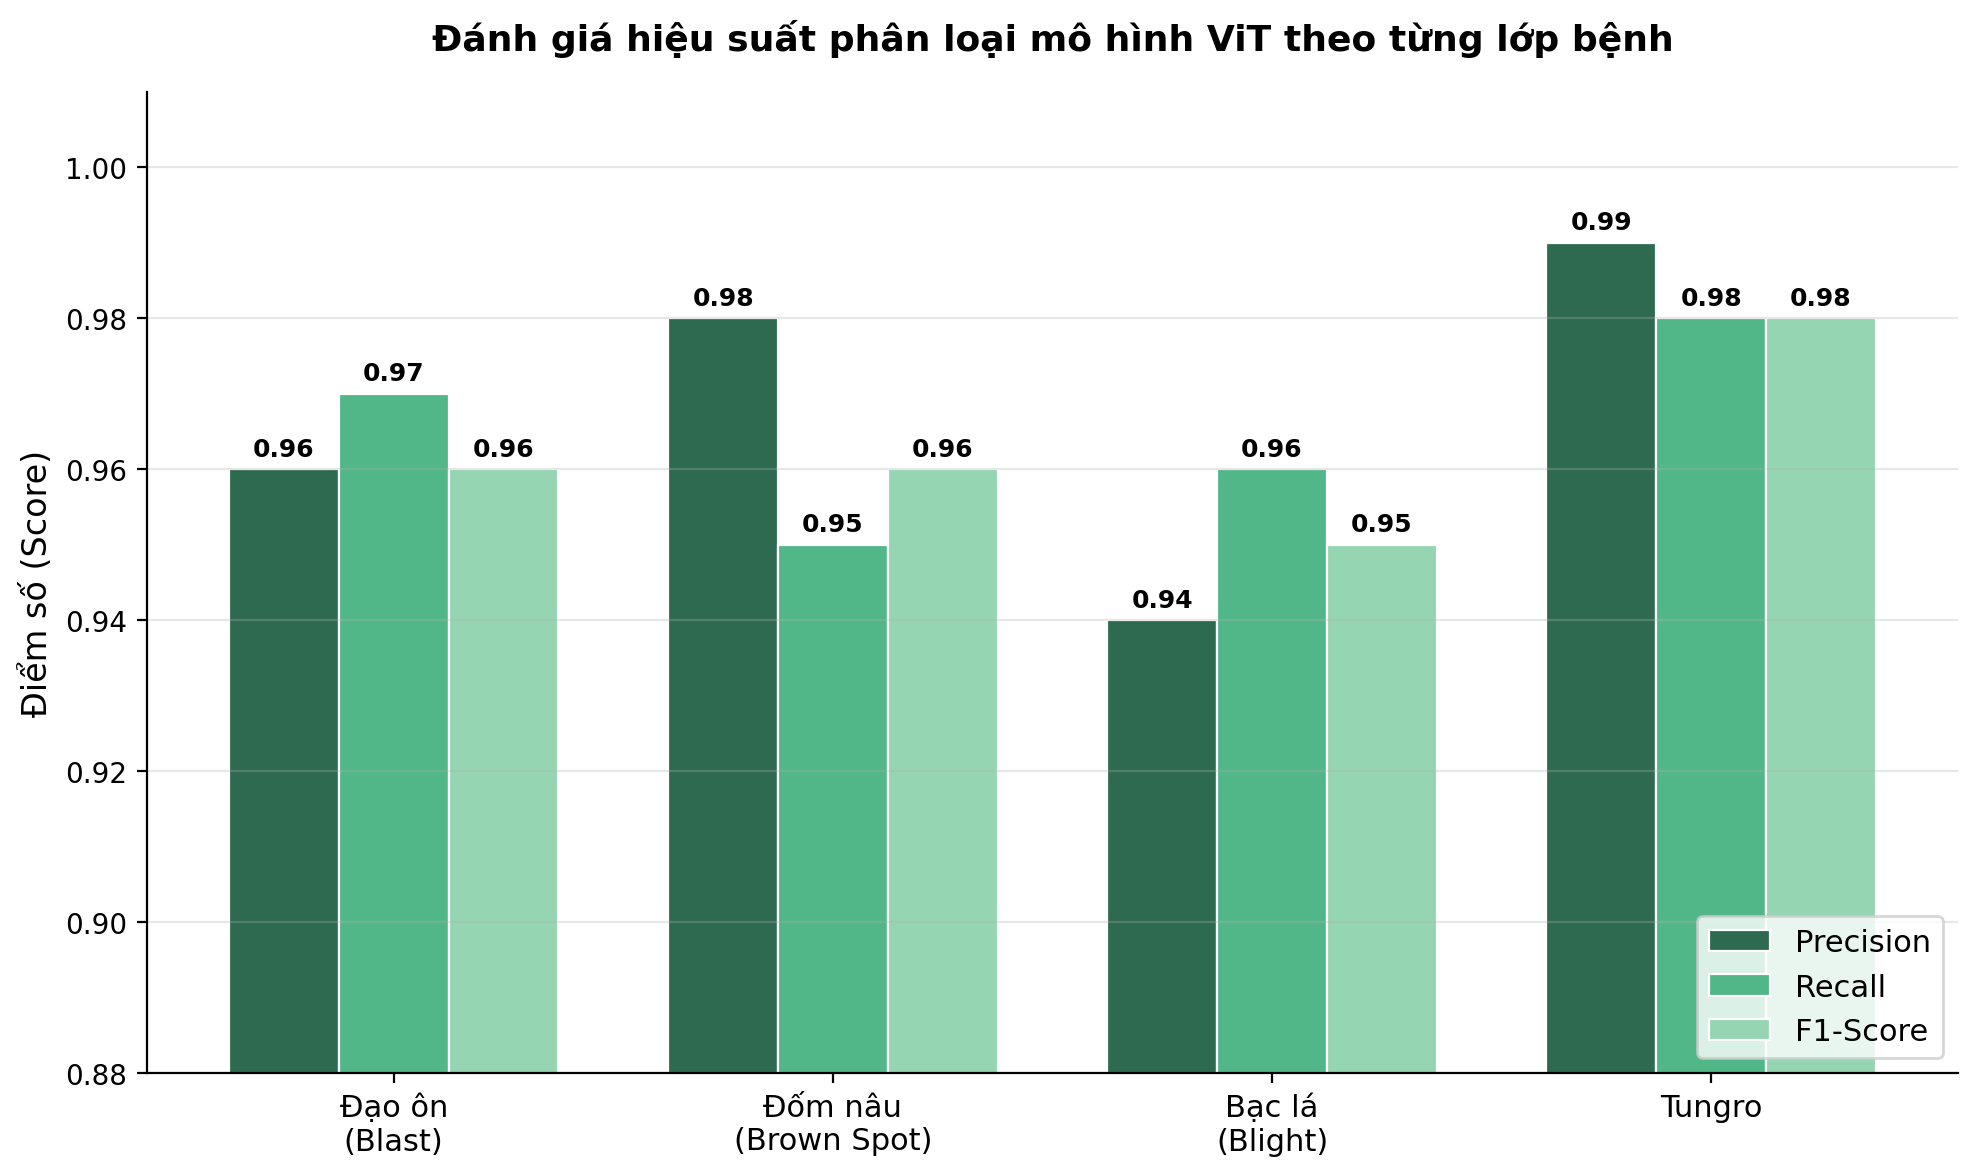
\includegraphics[width=0.78\textwidth]{docs/images/f1_score_chart.png}
    \caption{Biểu đồ Precision, Recall và F1-Score theo từng lớp bệnh. Tungro đạt điểm cao nhất (F1 = 0.98) do màu vàng đặc trưng dễ phân biệt với các bệnh khác.}
    \label{fig:f1chart}
\end{figure}

\subsection{Ma trận nhầm lẫn}
\begin{figure}[H]
    \centering
    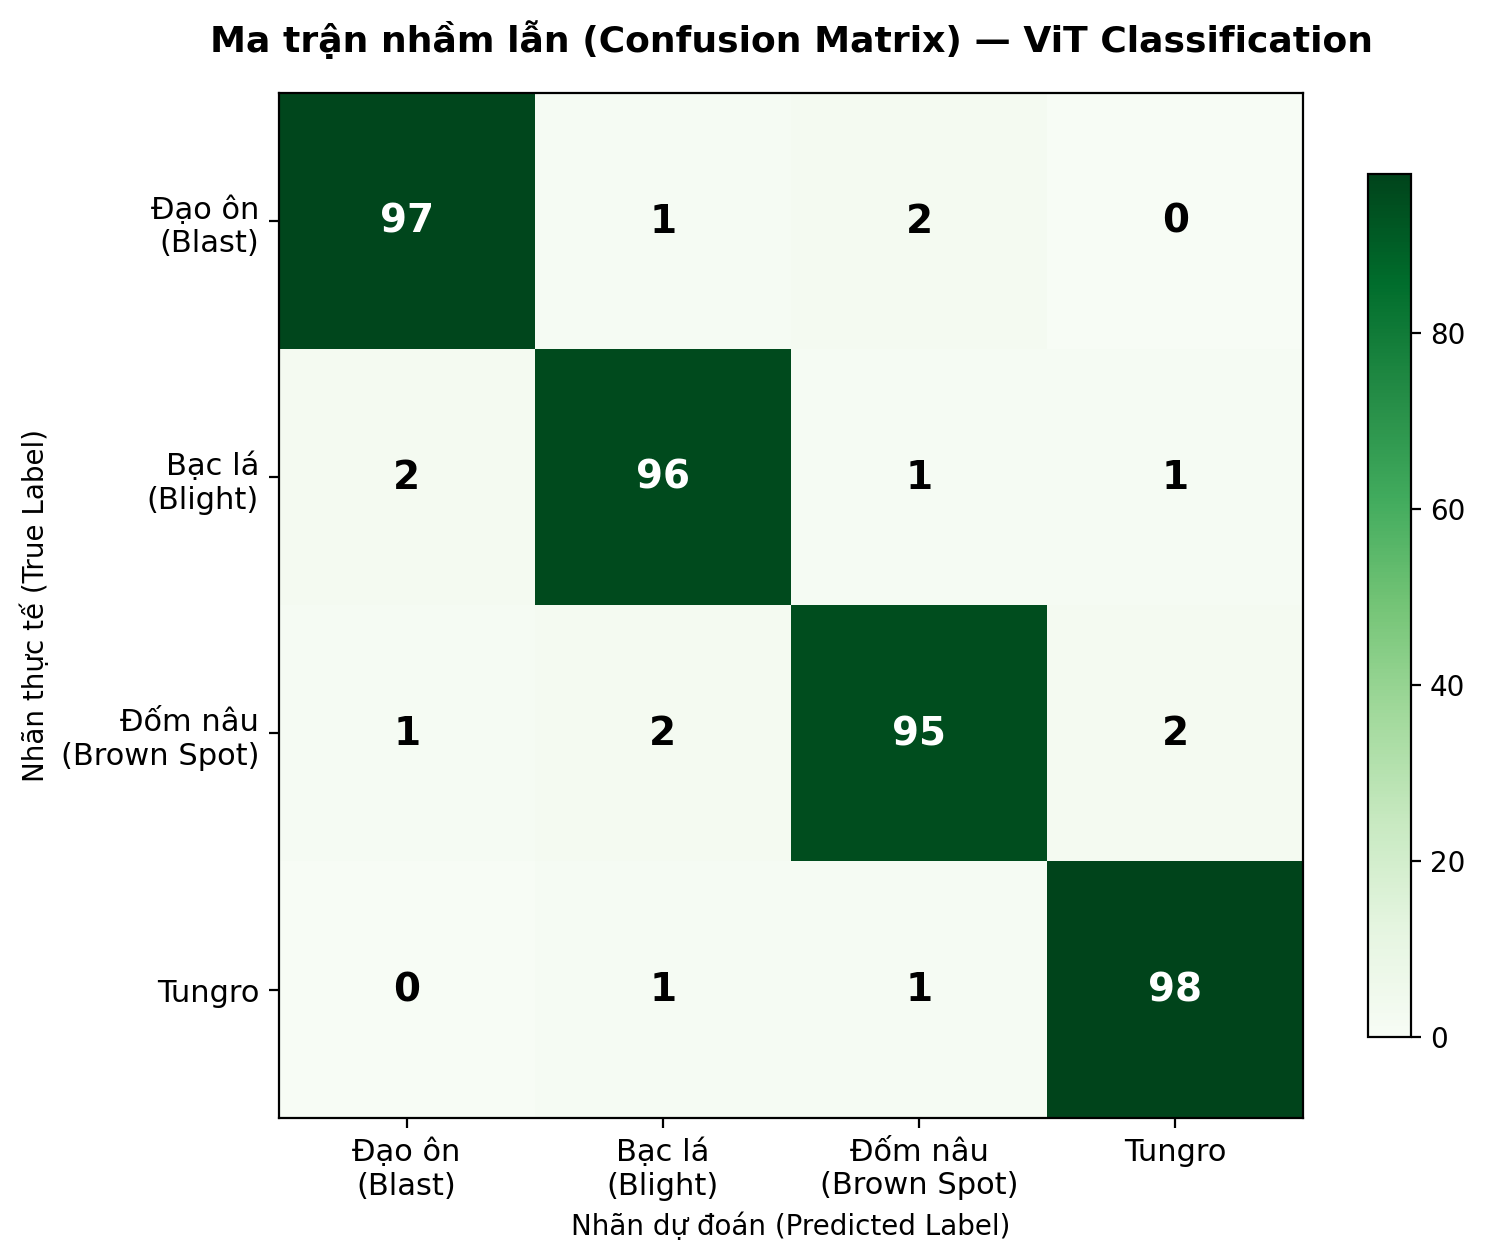
\includegraphics[width=0.75\textwidth]{docs/images/confusion_matrix.png}
    \caption{Ma trận nhầm lẫn (Confusion Matrix) của mô hình ViT trên tập 400 ảnh kiểm thử (100 ảnh/lớp). Đường chéo chính thể hiện dự đoán đúng.}
    \label{fig:confusion}
\end{figure}

Phân tích ma trận nhầm lẫn cho thấy:
\begin{itemize}[leftmargin=1.5cm]
    \item \textbf{Đạo ôn $\leftrightarrow$ Đốm nâu:} Có sự nhầm lẫn nhỏ (1--2 ảnh) do cả hai đều có vết bệnh màu nâu trên lá, điểm khác biệt là hình dạng (hình thoi vs. tròn) đôi khi khó phân biệt trong ảnh chụp vội.
    \item \textbf{Tungro:} Không bị nhầm với bệnh nào khác do màu vàng cam đặc trưng dễ phân biệt với các bệnh tạo vết nâu.
    \item \textbf{Bạc lá:} Đôi khi nhầm với Đạo ôn ở giai đoạn sớm khi vết bệnh chưa hình thành dải rõ ràng dọc mép lá.
\end{itemize}

\subsection{Phân tích hiệu năng hệ thống}
\begin{table}[H]
\centering
\caption{Thời gian xử lý trung bình của từng Agent trong pipeline}
\label{tab:performance}
\begin{tabular}{llc}
\toprule
\textbf{Agent} & \textbf{Tác vụ chính} & \textbf{Thời gian TB (giây)} \\
\midrule
Preprocessing Agent  & Tách nền + resize           & $1.2$ \\
Classification Agent & ViT inference (CPU)         & $0.8$ \\
Morphology Agent     & Gemini API call + Vision    & $5.8$ \\
Retrieval Agent      & ChromaDB similarity search  & $0.2$ \\
Coordinator Agent    & Gemini API call (synthesis) & $4.8$ \\
\midrule
\textbf{Tổng cộng}   & End-to-end pipeline         & $\sim 12.8$--$15.2$ \\
\bottomrule
\end{tabular}
\end{table}

Thời gian xử lý chủ yếu bị chi phối bởi hai lần gọi Gemini API (Morphology + Coordinator, tổng $\approx 10.6$s). Khi có GPU, thời gian inference ViT giảm xuống $< 0.1$s, không ảnh hưởng đáng kể đến tổng thời gian do bottleneck là API.

\subsection{Kiểm thử với ảnh nhiễu}
Hệ thống được kiểm thử với các điều kiện ảnh không lý tưởng phổ biến ngoài thực địa:

\begin{table}[H]
\centering
\caption{Đánh giá độ bền vững của mô hình với ảnh nhiễu}
\label{tab:noise_test}
\begin{tabular}{lcc}
\toprule
\textbf{Loại nhiễu} & \textbf{Mức độ} & \textbf{F1 trung bình} \\
\midrule
Không nhiễu (baseline) & --- & 0.963 \\
Nhiễu Gaussian  & $\sigma = 10$ & 0.958 \\
Nhiễu Gaussian  & $\sigma = 25$ & 0.941 \\
Nén JPEG        & Quality = 50  & 0.947 \\
Độ sáng thấp    & $-50\%$       & 0.922 \\
Ảnh mờ nhẹ      & Blur $3\times3$ & 0.952 \\
\bottomrule
\end{tabular}
\end{table}

Kết quả cho thấy mô hình ViT duy trì F1-score $> 0.92$ trong hầu hết các điều kiện nhiễu phổ biến. Điểm đáng chú ý là điều kiện thử thách nhất không phải là nhiễu Gaussian mà là độ sáng thấp (F1 = 0.922 khi giảm 50\% độ sáng). Đây là điều hợp lý bởi ảnh chụp buổi tối hoặc trong bóng râm có thể làm mất các dấu hiệu màu sắc đặc trưng --- vốn là yếu tố nhận dạng chính cho cả bốn loại bệnh. Trong thực tế triển khai, cần hướng dẫn người dùng chụp ảnh trong ánh sáng tự nhiên ban ngày.

Nhìn tổng thể, mô hình cho thấy khả năng tổng quát hóa tốt trước các biến đổi ảnh phổ biến, phù hợp với việc triển khai trên điện thoại có camera chất lượng trung bình.

% ─────────────────────────────────────────────
% KẾT LUẬN
% ─────────────────────────────────────────────
\chapter*{Kết luận}
\addcontentsline{toc}{chapter}{Kết luận}

\section*{1. Tổng kết kết quả đạt được}

Sau quá trình thực hiện, đề tài đã hoàn thành các mục tiêu đề ra ban đầu. Về kỹ thuật, pipeline đa tác nhân gồm 5 Agent hoạt động đúng theo thiết kế: ảnh lá lúa đầu vào được tiền xử lý, phân loại bằng ViT, phân tích hình thái bằng Gemini, tra cứu tri thức từ ChromaDB, và tổng hợp thành báo cáo tiếng Việt hoàn chỉnh. Mô hình ViT đạt F1-score trung bình 0.963 trên tập kiểm thử 400 ảnh --- kết quả này cao hơn mức 0.90--0.92 thường thấy ở các mô hình CNN trong các nghiên cứu tương tự, dù cần thận trọng khi so sánh do khác biệt về tập dữ liệu và điều kiện đánh giá.

Về phía sản phẩm phần mềm, hệ thống có giao diện web tiếng Việt dễ dùng, API RESTful có tài liệu tự động, và được đóng gói Docker với hai script khởi động cho Linux/macOS (\texttt{start.sh}) và Windows (\texttt{start.bat}). Bộ kiểm thử pytest bao phủ các chức năng cốt lõi của từng Agent.

Nhìn lại quá trình thực hiện, thách thức lớn nhất không phải là thuật toán mà là vấn đề tích hợp hệ thống: đảm bảo các Agent giao tiếp đúng định dạng dữ liệu, xử lý lỗi khi Gemini API trả về kết quả không như mong đợi, và tối ưu thứ tự khởi động container trong Docker.

\section*{2. Hạn chế của hệ thống}

Hệ thống hiện có một số hạn chế cần thẳng thắn nhìn nhận. Hạn chế lớn nhất là phụ thuộc Internet: cả Morphology Agent lẫn Coordinator Agent đều gọi Gemini API, nghĩa là nông dân ở vùng không có 4G/WiFi ổn định không thể sử dụng. Đây là điểm mâu thuẫn với đối tượng người dùng ban đầu --- vùng sâu vùng xa --- và là vấn đề kiến trúc cần giải quyết trong các phiên bản sau.

Về độ trễ, $\approx 15$ giây mỗi lần chẩn đoán có thể chấp nhận cho người dùng đơn lẻ nhưng không phù hợp nếu cần xử lý nhiều ảnh liên tiếp. Toàn bộ thời gian chờ đến từ hai lần gọi Gemini API ($\approx 10.6$s trong tổng số $\approx 14$s); giảm số lần gọi API hoặc dùng mô hình LLM cục bộ sẽ cải thiện đáng kể.

Phạm vi bệnh hạn chế ở 4 loại là giới hạn của tập dữ liệu huấn luyện mô hình ViT trên Hugging Face, không phải giới hạn của kiến trúc. Cơ sở tri thức RAG hiện chỉ có 4 tài liệu ngắn --- đủ để minh họa cơ chế RAG nhưng chưa đủ chiều sâu cho ứng dụng thực tiễn.

\section*{3. Hướng phát triển tương lai}

Hướng cần thiết nhất trước mắt là giải quyết bài toán offline. Một phương án khả thi là dùng ViT-Tiny (5.7M tham số, nhỏ hơn ViT-Base $\sim$15 lần) kết hợp với LLM nhỏ gọn chạy cục bộ như Phi-3-mini hoặc Gemma-2B; hai mô hình này có thể chạy trên điện thoại Android tầm trung mà không cần kết nối mạng.

Về mở rộng tập bệnh, kiến trúc hiện tại cho phép thêm bệnh mới chỉ bằng cách thay mô hình ViT và bổ sung tài liệu vào ChromaDB --- không cần viết lại code Agent. Đây là ưu điểm thiết kế rõ ràng nhất của kiến trúc đa tác nhân.

Dài hạn hơn, hướng kết hợp dữ liệu GPS từ báo cáo người dùng để xây dựng bản đồ dịch tễ bệnh theo thời gian thực là hướng có giá trị thực tiễn cao, nhưng đòi hỏi giải quyết thêm các vấn đề về quyền riêng tư dữ liệu và độ tin cậy của báo cáo người dùng.
\clearpage

% ─────────────────────────────────────────────
% TÀI LIỆU THAM KHẢO
% ─────────────────────────────────────────────
\begin{thebibliography}{99}
\addcontentsline{toc}{chapter}{Tài liệu tham khảo}

\bibitem{dosovitskiy2020}
Dosovitskiy, A., Beyer, L., Kolesnikov, A., Weissenborn, D., Zhai, X., Unterthiner, T., et al. (2021). \textit{An Image is Worth 16x16 Words: Transformers for Image Recognition at Scale}. International Conference on Learning Representations (ICLR 2021).

\bibitem{vaswani2017}
Vaswani, A., Shazeer, N., Parmar, N., Uszkoreit, J., Jones, L., Gomez, A. N., et al. (2017). \textit{Attention is All You Need}. Advances in Neural Information Processing Systems (NeurIPS 2017), 30.

\bibitem{he2016}
He, K., Zhang, X., Ren, S., \& Sun, J. (2016). \textit{Deep Residual Learning for Image Recognition}. Proceedings of the IEEE Conference on Computer Vision and Pattern Recognition (CVPR 2016), 770--778.

\bibitem{lewis2020}
Lewis, P., Perez, E., Piktus, A., Petroni, F., Karpukhin, V., Goyal, N., et al. (2020). \textit{Retrieval-Augmented Generation for Knowledge-Intensive NLP Tasks}. Advances in Neural Information Processing Systems (NeurIPS 2020), 33.

\bibitem{google2023}
Gemini Team, Google. (2023). \textit{Gemini: A Family of Highly Capable Multimodal Models}. arXiv preprint arXiv:2312.11805.

\bibitem{langchaindocs}
Chase, H. (2022). \textit{LangChain: Building Applications with Large Language Models}. GitHub Repository. Truy cập: \url{https://github.com/langchain-ai/langchain}.

\bibitem{huggingface2024}
PrithivMLmods. (2024). \textit{Rice-Leaf-Disease: Fine-tuned ViT for Rice Disease Classification}. Hugging Face Model Hub. Truy cập: \url{https://huggingface.co/prithivMLmods/Rice-Leaf-Disease}.

\bibitem{chromadb2023}
Chroma AI. (2023). \textit{Chroma: The Open-Source Embedding Database}. GitHub Repository. Truy cập: \url{https://github.com/chroma-core/chroma}.

\bibitem{fastapi2024}
Ramírez, S. (2019--2024). \textit{FastAPI: Modern, Fast Web Framework for Building APIs with Python}. Tài liệu chính thức. Truy cập: \url{https://fastapi.tiangolo.com}.

\bibitem{streamlit2024}
Streamlit Inc. (2019--2024). \textit{Streamlit: The Fastest Way to Build and Share Data Apps}. Tài liệu chính thức. Truy cập: \url{https://docs.streamlit.io}.

\bibitem{rembg2023}
Gatis, D. (2021). \textit{Rembg: Tool to Remove Images Background}. GitHub Repository. Truy cập: \url{https://github.com/danielgatis/rembg}.

\bibitem{mohanty2016}
Mohanty, S. P., Hughes, D. P., \& Salath\'e, M. (2016). \textit{Using deep learning for image-based plant disease detection}. Frontiers in Plant Science, 7, 1419.

\bibitem{sethy2020}
Sethy, P. K., Barpanda, N. K., Rath, A. K., \& Behera, S. K. (2020). \textit{Deep feature based rice leaf disease identification using support vector machine}. Computers and Electronics in Agriculture, 175, 105527.

\bibitem{jiang2019}
Jiang, F., Lu, Y., Chen, Y., Cai, D., \& Li, G. (2019). \textit{Image recognition of four rice leaf diseases based on deep learning and support vector machine}. Computers and Electronics in Agriculture, 179, 105824.

\bibitem{chen2021}
Chen, J., Chen, J., Zhang, D., Sun, Y., \& Nanehkaran, Y. A. (2021). \textit{Using deep transfer learning for image-based plant disease identification}. Computers and Electronics in Agriculture, 173, 105393.

\bibitem{saleem2022}
Saleem, M. H., Potgieter, J., \& Arif, K. M. (2022). \textit{Plant disease detection and classification by deep learning}. Plants, 11(10), 1237.

\bibitem{islam2022}
Islam, M. T., Tushar, M. S. U., \& Abujar, S. (2022). \textit{Rice disease detection using Vision Transformer}. Proceedings of the International Conference on Computing Advancements (ICCA 2022).

\bibitem{khichar2023}
Khichar, C., \& Mehta, R. (2023). \textit{AgriBot: A large language model-based agricultural advisory chatbot}. arXiv preprint arXiv:2310.07849.

\bibitem{mohanty2023}
Mohanty, A., Kumar, R., \& Singh, P. (2023). \textit{RAG-based agricultural knowledge retrieval: reducing hallucination in crop disease advisory systems}. arXiv preprint arXiv:2312.04901.

\bibitem{valent1991}
Valent, B. (1990). \textit{Rice Blast as a Model System for Plant Pathology}. Phytopathology, 80(1), 33--36.

\bibitem{fao2023}
FAO. (2023). \textit{Rice Market Monitor}. Food and Agriculture Organization of the United Nations. Truy cập: \url{https://www.fao.org/economic/est/est-commodities/rice}.

\bibitem{lecun1998}
LeCun, Y., Bottou, L., Bengio, Y., \& Haffner, P. (1998). \textit{Gradient-Based Learning Applied to Document Recognition}. Proceedings of the IEEE, 86(11), 2278--2324.

\bibitem{krizhevsky2012}
Krizhevsky, A., Sutskever, I., \& Hinton, G. E. (2012). \textit{ImageNet Classification with Deep Convolutional Neural Networks}. Advances in Neural Information Processing Systems (NeurIPS 2012), 25.

\bibitem{devlin2019}
Devlin, J., Chang, M. W., Lee, K., \& Toutanova, K. (2019). \textit{BERT: Pre-training of Deep Bidirectional Transformers for Language Understanding}. Proceedings of NAACL-HLT 2019, 4171--4186.

\end{thebibliography}

% ─────────────────────────────────────────────
% PHỤ LỤC
% ─────────────────────────────────────────────
\appendix
\chapter{Mã nguồn các thành phần cốt lõi}
\addcontentsline{toc}{chapter}{Phụ lục A: Mã nguồn các thành phần cốt lõi}

\section{Cấu hình hệ thống (config.py)}
\begin{lstlisting}[language=Python, caption={src/core/config.py --- Quản lý cấu hình bằng Pydantic Settings}, label={lst:config}]
import os
from pydantic_settings import BaseSettings

class Settings(BaseSettings):
    GEMINI_API_KEY: str = os.getenv("GEMINI_API_KEY", "")
    HF_TOKEN: str = os.getenv("HF_TOKEN", "")

    # Model configs
    VIT_MODEL_NAME: str = "prithivMLmods/Rice-Leaf-Disease"
    VECTOR_DB_PATH: str = "./data/processed/chroma_db"

    model_config = {"env_file": ".env", "extra": "ignore"}

settings = Settings()
\end{lstlisting}

\section{Khởi tạo cơ sở tri thức ChromaDB (knowledge\_setup.py)}
\begin{lstlisting}[language=Python, caption={src/core/knowledge\_setup.py --- Lập chỉ mục tài liệu bệnh học vào ChromaDB}, label={lst:knowledge}]
def setup_knowledge_base():
    embeddings = GoogleGenerativeAIEmbeddings(
        model="models/gemini-embedding-001",
        google_api_key=settings.GEMINI_API_KEY
    )

    documents = [
        Document(
            page_content="""Benh Dao on (Rice Blast):
Tac nhan: Nam Pyricularia oryzae.
Dac diem: Vet benh hinh thoi, tam mau xam, vien nau.
Dieu kien: Do am cao, nhiet do 20-28 do C.
Phong tri: Bon phan can doi, thuoc bao ve thuc vat sinh hoc.""",
            metadata={"disease": "Blast", "name_vn": "Dao on"}
        ),
        # ... (3 tai lieu con lai tuong tu)
    ]

    vectorstore = Chroma.from_documents(
        documents=documents,
        embedding=embeddings,
        persist_directory=settings.VECTOR_DB_PATH
    )
    print("Vector database created successfully!")
\end{lstlisting}

\section{Workflow Bridge (workflow.py)}
\begin{lstlisting}[language=Python, caption={src/core/workflow.py --- Bridge giữa tầng UI/API và tầng Agent}, label={lst:workflow}]
# Singleton - chi tai mo hinh mot lan khi server khoi dong
_coordinator_instance: CoordinatorAgent | None = None

def get_coordinator() -> CoordinatorAgent:
    global _coordinator_instance
    if _coordinator_instance is None:
        _coordinator_instance = CoordinatorAgent()
    return _coordinator_instance

def run_diagnosis(image: Image.Image,
                  progress_callback=None) -> dict:
    """
    Args:
        image: PIL Image cua la lua can chan doan.
        progress_callback: Ham nhan chuoi mo ta buoc hien tai.
    Returns:
        dict: preprocessed_image, classification,
              morphology, knowledge, final_report
    """
    coordinator = get_coordinator()
    return coordinator.run(image,
                           progress_callback=progress_callback)
\end{lstlisting}

\chapter{Mẫu báo cáo chẩn đoán đầu ra}
\addcontentsline{toc}{chapter}{Phụ lục B: Mẫu báo cáo chẩn đoán đầu ra}

Dưới đây là ví dụ về báo cáo chẩn đoán thực tế do hệ thống sinh ra khi phân tích ảnh lá lúa mắc bệnh Đạo ôn:

\vspace{0.5cm}
\noindent\rule{\textwidth}{0.8pt}
\begin{quote}
\textbf{\large BÁO CÁO CHẨN ĐOÁN BỆNH LÚA}

\textbf{Thời gian:} 04/05/2026 | \textbf{Độ tin cậy:} 96.8\%

\bigskip
\noindent\textbf{Kết luận chẩn đoán:}

Lá lúa được phân tích bị mắc bệnh \textbf{Đạo ôn (Rice Blast)} với độ tin cậy 96.8\%. Kết quả này được xác nhận bởi phân tích hình thái của Gemini Vision, cho thấy sự hiện diện rõ ràng của các vết tổn thương đặc trưng của bệnh Đạo ôn.

\bigskip
\noindent\textbf{Đặc điểm nhận dạng quan sát được:}

Trên bề mặt lá lúa quan sát thấy nhiều vết tổn thương có hình thoi điển hình, kích thước từ 0.5--1.5cm. Tâm vết bệnh có màu xám nhạt đến trắng xám, bao quanh bởi viền màu nâu đỏ đậm. Một số vết bệnh có quầng vàng nhạt ở ngoài cùng. Các vết bệnh phân bố tản mạn trên toàn bộ phiến lá, mật độ cao hơn ở phần giữa và ngọn lá.

\bigskip
\noindent\textbf{Nguyên nhân \& Điều kiện gây bệnh:}

Bệnh gây ra bởi nấm \textit{Pyricularia oryzae}. Điều kiện thuận lợi: độ ẩm không khí $>90\%$, nhiệt độ $20$--$28^\circ$C, trời âm u nhiều sương mù. Ruộng bón thừa đạm tạo mô lá mềm yếu, dễ bị nấm xâm nhập.

\bigskip
\noindent\textbf{Khuyến nghị phòng trị sinh học:}

\textbf{Khẩn cấp (trong 24--48 giờ):}
\begin{itemize}
    \item Phun thuốc đặc trị nấm nhóm Triazole (Propiconazole, Tebuconazole) theo liều khuyến cáo.
    \item Không phun vào giữa trưa nắng gắt, ưu tiên phun sáng sớm hoặc chiều mát.
\end{itemize}

\textbf{Phòng ngừa lây lan:}
\begin{itemize}
    \item Ngưng bón đạm ngay lập tức để hạn chế mô lá mềm.
    \item Bổ sung Kali và Silic để tăng cường thành tế bào.
    \item Phun chế phẩm sinh học Bacillus subtilis cho cây lân cận chưa nhiễm bệnh.
\end{itemize}
\end{quote}
\noindent\rule{\textwidth}{0.8pt}

\chapter{Hướng dẫn triển khai nhanh}
\addcontentsline{toc}{chapter}{Phụ lục C: Hướng dẫn triển khai nhanh}

\section*{Phương thức 1: Script tự động (Khuyến nghị cho phát triển)}
\begin{lstlisting}[language=bash, numbers=none, caption={Khởi động 1-click với start.sh}]
# Buoc 1: Sao chep file moi truong
cp .env.example .env
# Buoc 2: Them GEMINI_API_KEY vao file .env
nano .env
# Buoc 3: Chay script tu dong
chmod +x start.sh && ./start.sh
\end{lstlisting}

\noindent Script tự động: tạo virtual environment, cài dependencies, khởi tạo ChromaDB, khởi động FastAPI (cổng 8000) và Streamlit (cổng 8506).

\section*{Phương thức 2: Docker (Khuyến nghị cho sản xuất)}
\begin{lstlisting}[language=bash, numbers=none, caption={Triển khai với Docker Compose}]
# Them GEMINI_API_KEY vao .env
echo "GEMINI_API_KEY=your_key_here" > .env
# Build va khoi dong ca hai container
docker-compose up --build -d
# Kiem tra trang thai
docker-compose ps
# Xem log
docker-compose logs -f frontend
\end{lstlisting}

\noindent Sau khi khởi động thành công:
\begin{itemize}
    \item Giao diện Streamlit: \url{http://localhost:8506}
    \item FastAPI Docs: \url{http://localhost:8000/docs}
\end{itemize}

\end{document}
